%%%%%%%%%%%%%%%%%%%%%%%%%%%%%%%%%%%%%%%%%%%%%%%%%
%\chapter{Constraint Handling Methods}
%%%%%%%%%%%%%%%%%%%%%%%%%%%%%%%%%%%%%%%%%%%%%%%%%
%\section{Lumping-based methods}
\chapter{Numerical results}  \label{sec:results}


We implement an adjoint treatment for multicomponent oil-gas
compositional systems through use of a recently developed automatic
differentiation capability \citep{Younis:2010}. The application of automatic
differentiation in the context of Stanford's General Purpose Research Simulator
(AD-GPRS) \citep{Cao:Thesis}, a modular simulator with many advanced features,
enables us to construct a gradient-based optimization framework suitable for
use in compositional problems. Our formulation includes the treatment of
bound, linear and nonlinear constraints. In a discrete implementation, the 
governing equations for the so-called adjoint
system are constructed based on the discretized-in-time forward model
equations. 

We will present results for four different cases. All involve bound and
nonlinear constraints, and we will compare the performance of the two approaches
described above for treating the nonlinear constraints. Because our
gradient-based optimization will find only a local optimum, we run each case
nine times, using a different initial guess for the well controls. Each initial
guess corresponds to a combination of BHPs from the set $\{p_I^u,p_I^l,p_I^a\}$
for the injectors and from the set $\{p_P^u,p_P^l,p_P^a\}$ for the producers,
where $p^u$, $p^l$ and $p^a$ designate the upper and lower limits on the
initial BHPs, and the average between these limits, respectively. We set
$p^l=p_{init}+1~{\rm bar}$ for the injectors and $p^u=p_{init}-1~{\rm bar}$
for the producers, where $p_{init}$ is the initial reservoir pressure. Note
that these `limits' are simply used to prescribe initial guesses for the
optimization -- they are not related to the actual BHP bound constraints.
For clarity, we will refer to each case by the number of the corresponding
run, as listed in Table~\ref{table:InitialGuesses}.



\begin{table}
\centering
\caption{Resulted objective values for every continuity step with respect to permeability 
for all benchmarks.}
\begin{tabular}{cccc}
\toprule
Run & SPE10TOP 1000D & SPE10TOP 3000D & Pi 256D   \\[2pt]
\midrule
1 & $5.443892E+05$ & $6.642702E+05$ & $1.252661E+05$  \\
2 & $5.631894E+05$ & $6.706731E+05$ & $1.252819E+05$ \\
3 & $5.873230E+05$  & $6.756695E+05$    & $1.244174E+05$ \\
4 & $5.986247E+05$ & $6.763321E+05$   & $1.242821E+05$ \\
5 & $5.998848E+05$  & $6.760098E+05$   & $1.241929E+05$  \\
6 & $5.962259E+05$  & $6.782397E+05$   & $1.240130E+05$   \\
7 & $5.909467E+05$  & $6.762526E+05$   & $1.242663E+05$  \\
8 & $5.850723E+05$  & $6.724442E+05$   & $1.241064E+05$  \\
9 & $5.775845E+05$  & $6.667619E+05$   & $1.240303E+05$  \\
10 & $5.688990E+05$  & $6.584114E+05$   & $1.234992E+05$   \\
11 & $5.594653E+05$  & $6.501344E+05$   & $1.229465E+05$  \\
12 & $5.507783E+05$  & $6.427540E+05$   & $1.229158E+05$  \\
13 & $5.422065E+05$  & $6.365637E+05$   & $1.226925E+05$  \\
14 & $5.339263E+05$  & $[p_I^a, p_P^a]$   & $1.225814E+05$   \\
15 & $5.256504E+05$  & $[p_I^a, p_P^a]$   & $1.221619E+05$  \\
16 & $5.180703E+05$  & $[p_I^a, p_P^a]$   & $1.217791E+05$  \\
17 & $5.120160E+05$  & $[p_I^a, p_P^a]$   & $1.214983E+05$   \\
18 & $5.071502E+05$  & $[p_I^a, p_P^a]$   & $1.212952E+05$  \\
19 & $5.044022E+05$  & $[p_I^a, p_P^a]$   & $1.211731E+05$  \\
20 & $5.033963E+05$  & $[p_I^a, p_P^a]$   & $1.211338E+05$  \\[2pt]
20* & $5.089974E+05$  & $6.018453E+05$   & $1.188555E+05$  \\[2pt]
\bottomrule
\end{tabular}
  \label{table:InitialGuesses}
\end{table}

% \begin{table}
% \centering
% \caption{Resulted objective values of the SPE10 benchmark produced for 3000 days.}
% \begin{tabular}{cc}
% \toprule
% Run & Objective value    \\[2pt]
% \midrule
% 1 & $6.642702E+05$ \\
% 2 & $6.706731E+05$ \\
% 3 & $111$ \\
% 4 & $[p_I^a, p_P^l]$ \\
% 5 & $[p_I^a, p_P^a]$ \\
% 6 & $[p_I^a, p_P^u]$ \\
% 7 & $[p_I^u, p_P^l]$ \\
% 8 & $[p_I^u, p_P^a]$ \\
% 9 & $[p_I^u, p_P^u]$ \\[2pt]
% \bottomrule
% \end{tabular}
%   \label{table:InitialGuesses}
% \end{table}
% 
% \begin{table}
% \centering
% \caption{Resulted objective values of the Pi benchmark produced for 256 days.}
% \begin{tabular}{cc}
% \toprule
% Run & Objective value    \\[2pt]
% \midrule
% 1 & $1.252661E+05$ \\
% 2 & $1.252819E+05$ \\
% 3 & $1.244174E+05$ \\
% 4c \\
% 5 & $[p_I^a, p_P^a]$ \\
% 6 & $[p_I^a, p_P^u]$ \\
% 7 & $[p_I^u, p_P^l]$ \\
% 8 & $[p_I^u, p_P^a]$ \\
% 9 & $[p_I^u, p_P^u]$ \\[2pt]
% \bottomrule
% \end{tabular}
%   \label{table:InitialGuesses}
% \end{table}
% 
% 
% 
% 
% \begin{table}
% \centering
% \caption{Initial guesses for the optimizations for all
%          cases considered.}
% \begin{tabular}{cc}
% \toprule
% Run & Initial guess    \\[2pt]
% \midrule
% 1 & $[p_I^l, p_P^l]$ \\
% 2 & $[p_I^l, p_P^a]$ \\
% 3 & $[p_I^l, p_P^u]$ \\
% 4 & $[p_I^a, p_P^l]$ \\
% 5 & $[p_I^a, p_P^a]$ \\
% 6 & $[p_I^a, p_P^u]$ \\
% 7 & $[p_I^u, p_P^l]$ \\
% 8 & $[p_I^u, p_P^a]$ \\
% 9 & $[p_I^u, p_P^u]$ \\[2pt]
% \bottomrule
% \end{tabular}
%   \label{table:InitialGuesses}
% \end{table}

\begin{figure}[htb]
\centering
\begin {tabular}{@{}cccc@{}}
 
\includegraphics[width=0.23\textwidth]{figures/VisitScreenshots/SPE1000/SPE1000_PERM_t01.png} &
 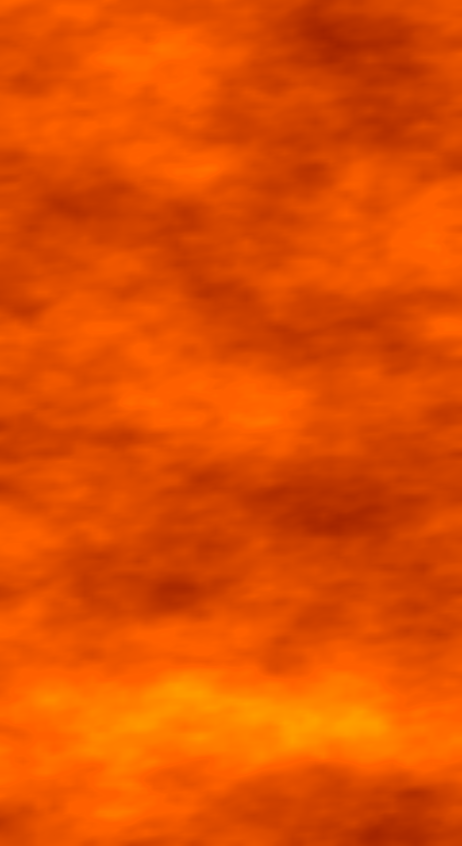
\includegraphics[width=0.23\textwidth]{figures/VisitScreenshots/SPE1000/SPE1000_PERM_t02.png} &
 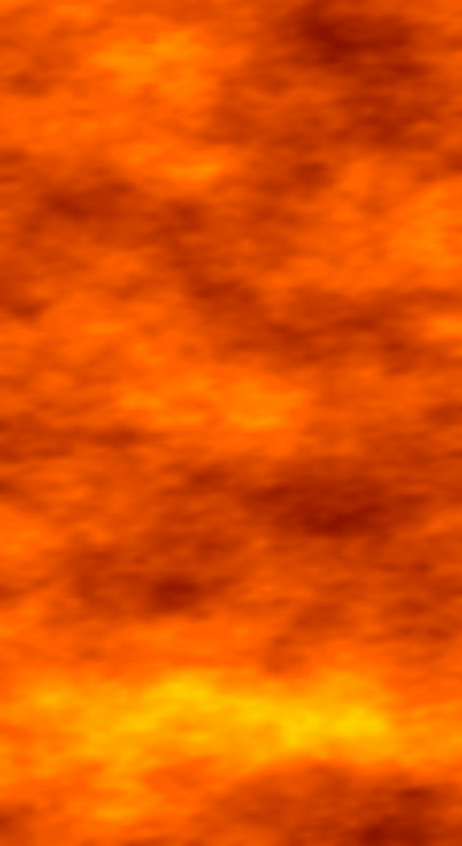
\includegraphics[width=0.23\textwidth]{figures/VisitScreenshots/SPE1000/SPE1000_PERM_t03.png} &
 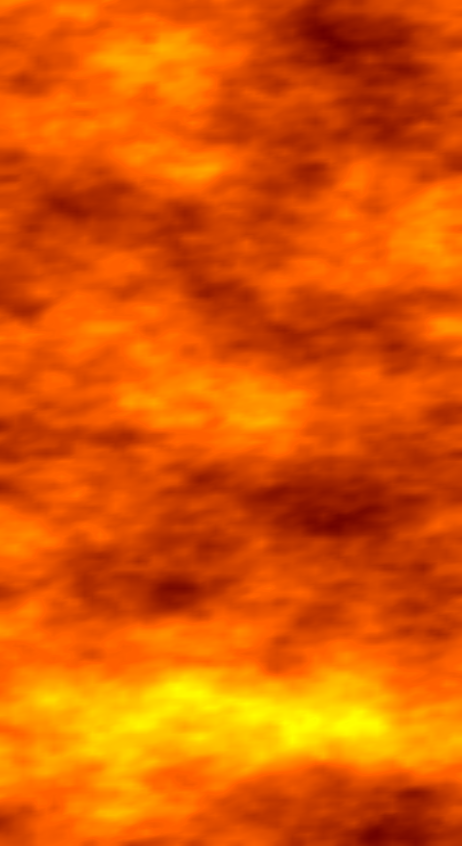
\includegraphics[width=0.23\textwidth]{figures/VisitScreenshots/SPE1000/SPE1000_PERM_t04.png} \\
 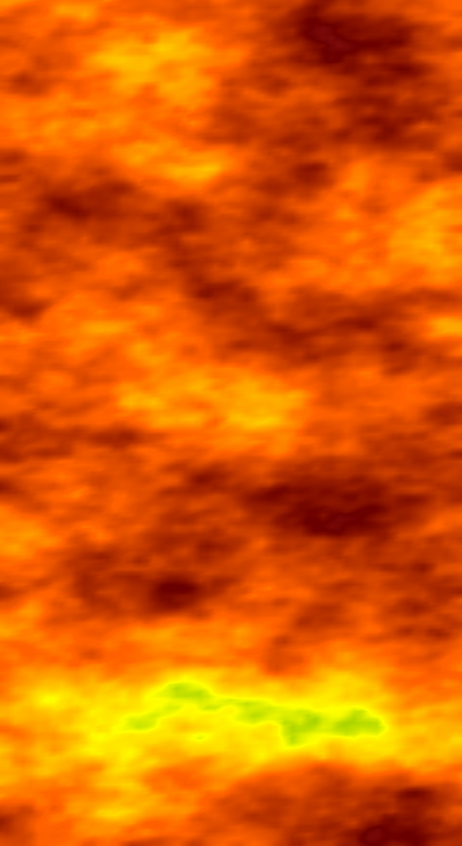
\includegraphics[width=0.23\textwidth]{figures/VisitScreenshots/SPE1000/SPE1000_PERM_t05.png} &
 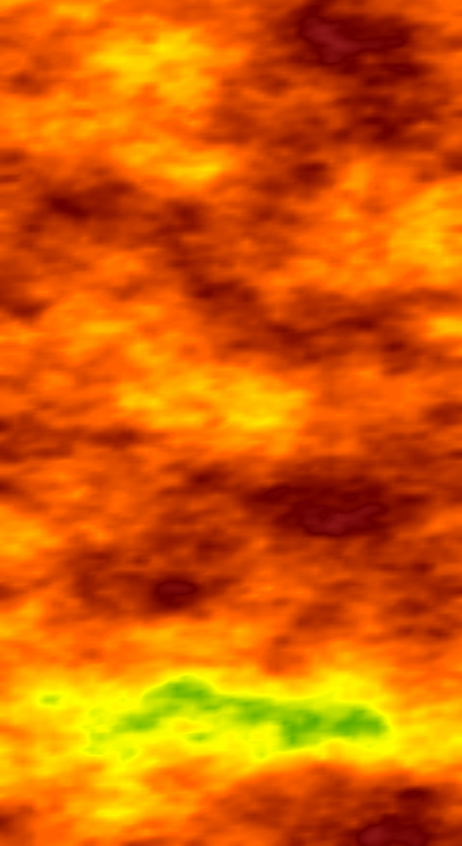
\includegraphics[width=0.23\textwidth]{figures/VisitScreenshots/SPE1000/SPE1000_PERM_t06.png} &
 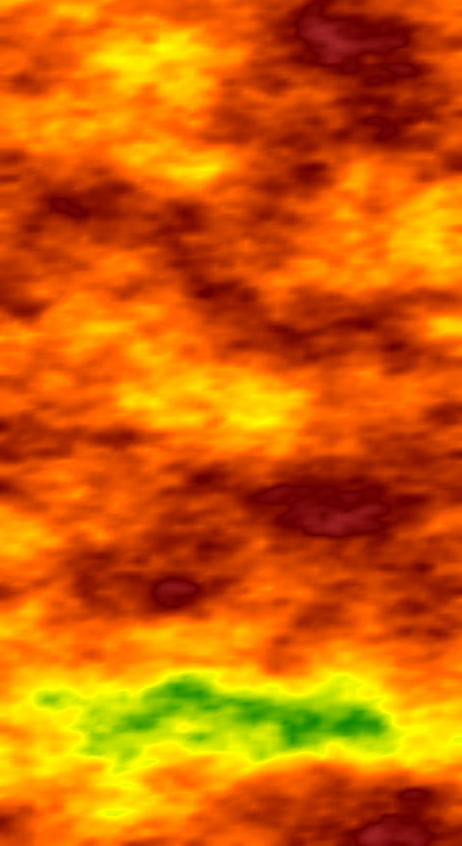
\includegraphics[width=0.23\textwidth]{figures/VisitScreenshots/SPE1000/SPE1000_PERM_t07.png} &
 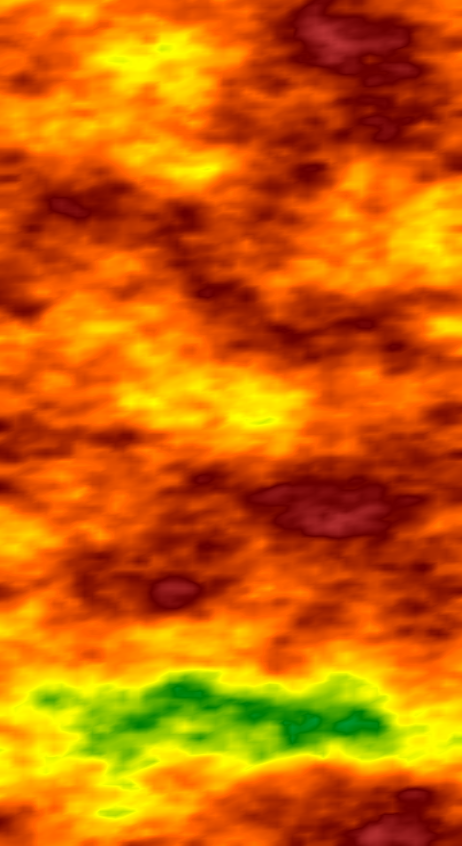
\includegraphics[width=0.23\textwidth]{figures/VisitScreenshots/SPE1000/SPE1000_PERM_t08.png} \\
 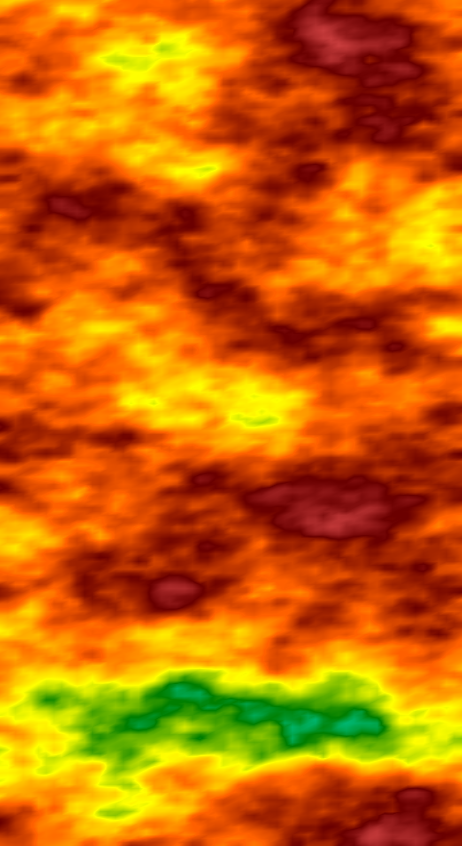
\includegraphics[width=0.23\textwidth]{figures/VisitScreenshots/SPE1000/SPE1000_PERM_t09.png} &
 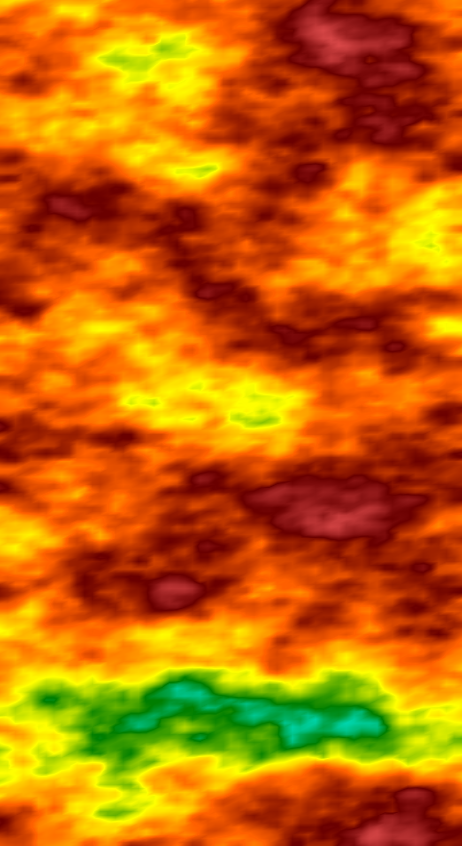
\includegraphics[width=0.23\textwidth]{figures/VisitScreenshots/SPE1000/SPE1000_PERM_t10.png} &
 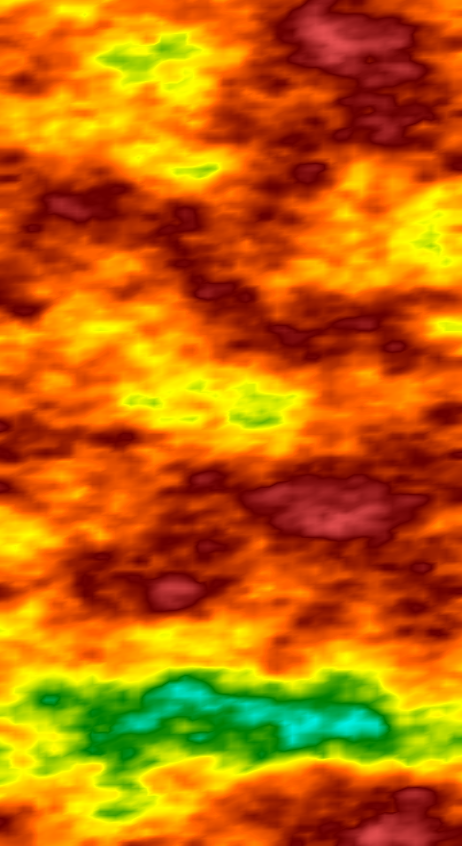
\includegraphics[width=0.23\textwidth]{figures/VisitScreenshots/SPE1000/SPE1000_PERM_t11.png} &
 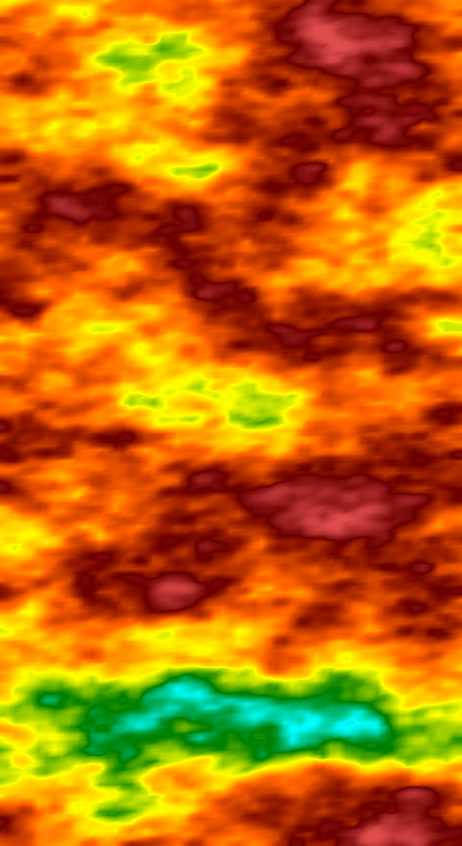
\includegraphics[width=0.23\textwidth]{figures/VisitScreenshots/SPE1000/SPE1000_PERM_t12.png} \\
 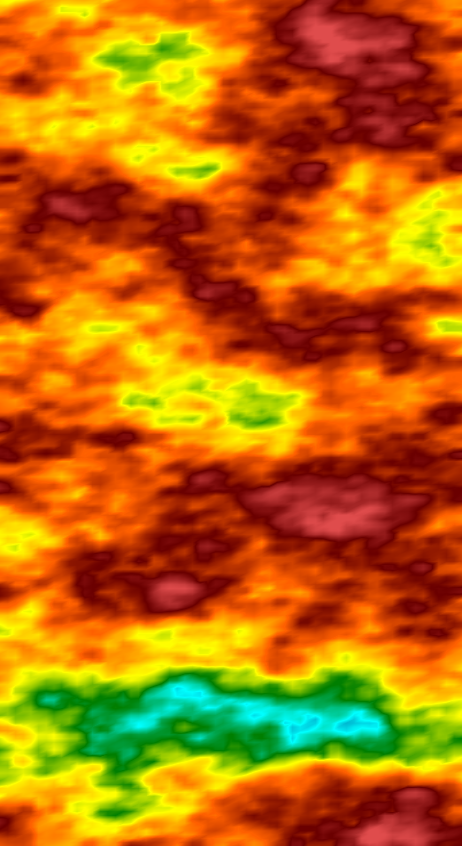
\includegraphics[width=0.23\textwidth]{figures/VisitScreenshots/SPE1000/SPE1000_PERM_t13.png} &
 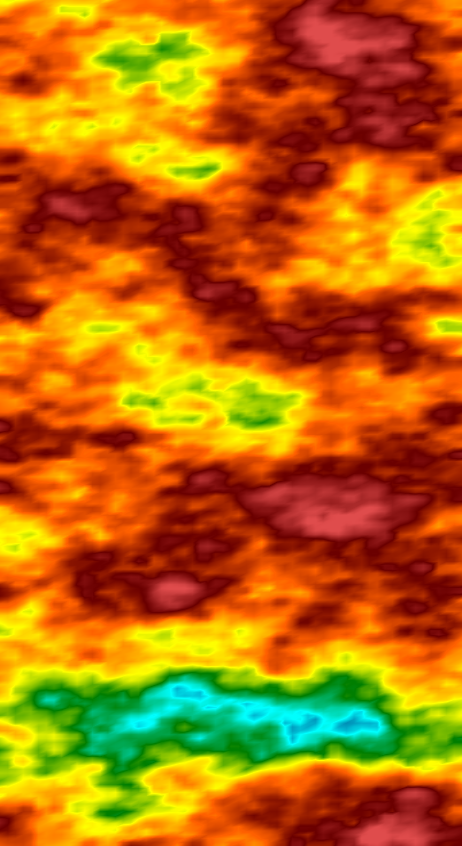
\includegraphics[width=0.23\textwidth]{figures/VisitScreenshots/SPE1000/SPE1000_PERM_t14.png} &
 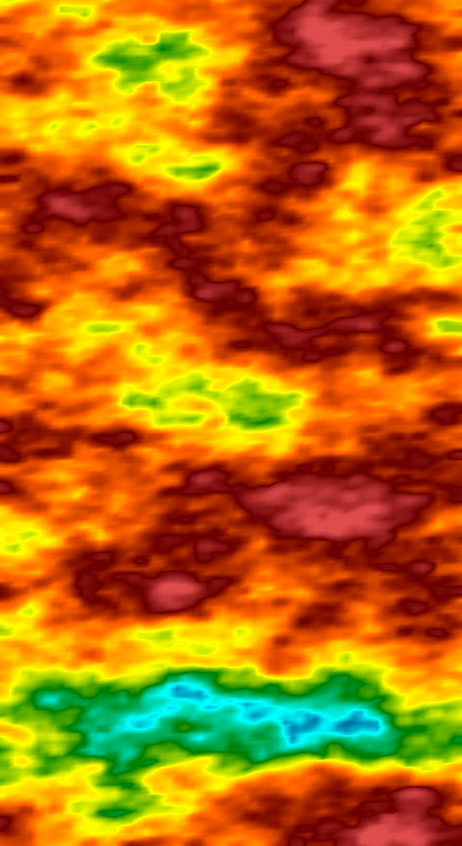
\includegraphics[width=0.23\textwidth]{figures/VisitScreenshots/SPE1000/SPE1000_PERM_t15.png} &
 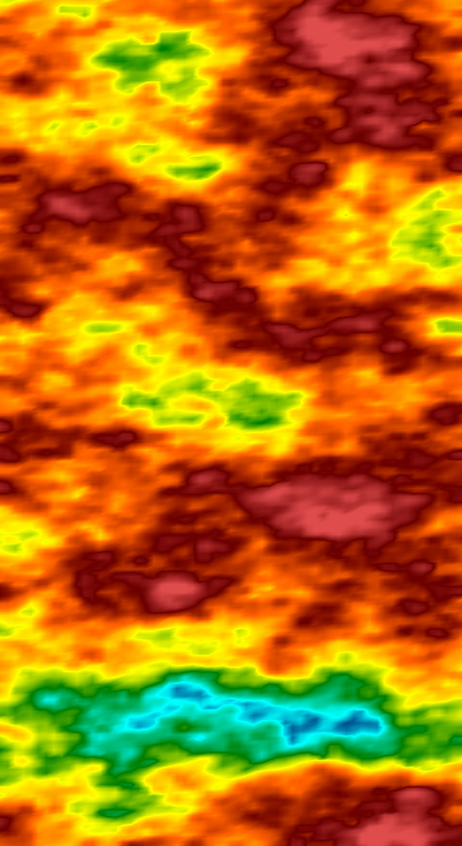
\includegraphics[width=0.23\textwidth]{figures/VisitScreenshots/SPE1000/SPE1000_PERM_t16.png} \\
%  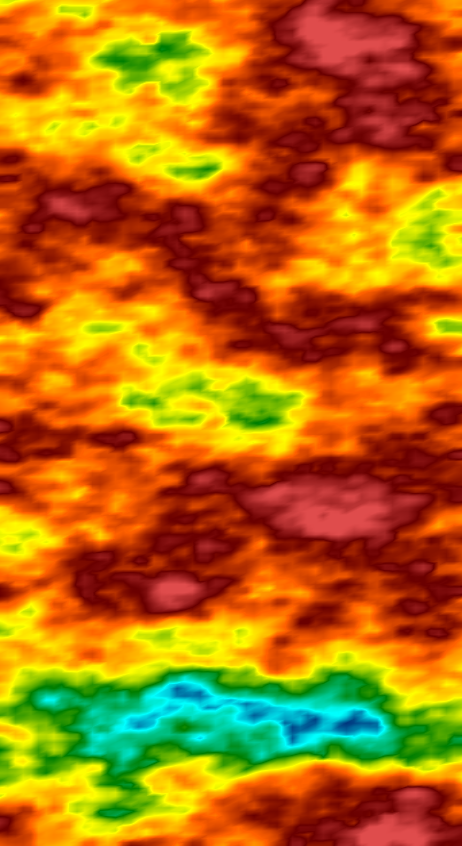
\includegraphics[width=0.23\textwidth]{figures/VisitScreenshots/SPE1000/SPE1000_PERM_t17.png} &
%  
\includegraphics[width=0.23\textwidth]{figures/VisitScreenshots/SPE1000/SPE1000_PERM_t01.png} &
%  
\includegraphics[width=0.23\textwidth]{figures/VisitScreenshots/SPE1000/SPE1000_PERM_t01.png} &
%  
\includegraphics[width=0.23\textwidth]{figures/VisitScreenshots/SPE1000/SPE1000_PERM_t01.png} \\
\multicolumn{4}{c}%{ 
\includegraphics[width=0.23\textwidth]{figures/VisitScreenshots/SPE1000/SPE1000_PERM_t01.png} }

\end {tabular}
\caption {hgchgm}

% \begin{subfigure}{0.5\textwidth}
% 
\includegraphics[width=0.9\linewidth, height=5cm]{figures/VisitScreenshots/SPE1000/SPE1000_PERM_t01.png} 
% \caption{Permeability}
% \label{fig:subim1}
% \end{subfigure}
% \begin{subfigure}{0.5\textwidth}
% 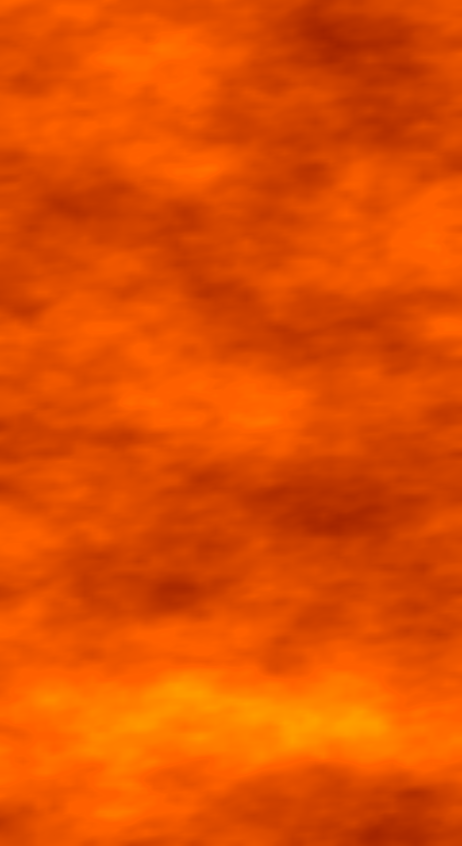
\includegraphics[width=0.9\linewidth, height=5cm]{figures/VisitScreenshots/SPE1000/SPE1000_PERM_t02.png}
% \caption{Oil saturation}
% \label{fig:subim2}
% \end{subfigure}
% \begin{subfigure}{0.5\textwidth}
% 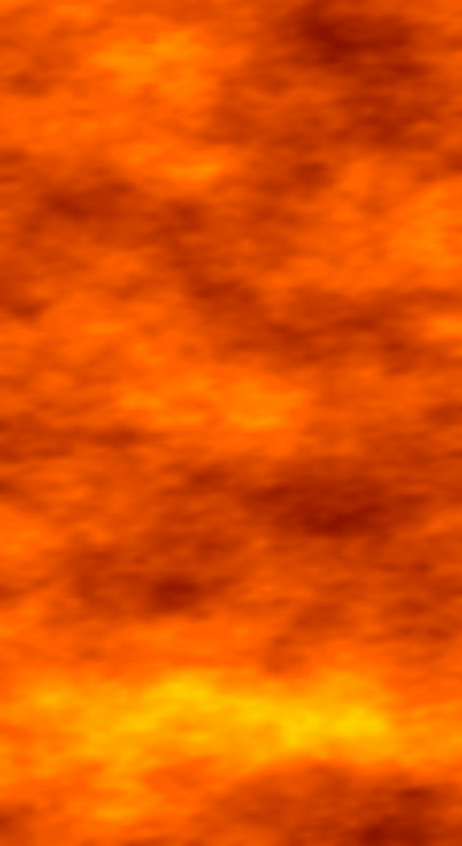
\includegraphics[width=0.9\linewidth, height=5cm]{figures/VisitScreenshots/SPE1000/SPE1000_PERM_t03.png}
% \caption{Oil saturation}
% \label{fig:subim2}
% \end{subfigure}
% \caption{Step 1 out of 20 for the SPE10 top layer, after 3000 days, .}
% \label{fig:image2}
 \end{figure}



\subsection{Example 1 - $\Pi$ obstacle}

In the first example we maximize cumulative oil recovery under CO$_2$ injection. The two-dimensional geological model is depicted in Fig.~\ref{fig:PImodelPermeabilityMapAndWells}. A $\Pi$-shaped region is located at the center of a homogeneous reservoir. The model is discretized on a grid of dimensions $80\times80$. The permeability in most of the domain (red cells) is set to 4000~mD, while the permeability for the blue cells that comprise the $\Pi$-shaped region is set to $10^{-4}$~mD. In all of our examples we describe the permeability with a diagonal tensor: $\tens{K} = \it{diag}(\tens{k}_x, \tens{k}_y, \tens{k}_z)$; here, in addition, the permeability is isotropic and uniform within each of the regions. Four injection wells are placed at the corners of the model, and the single production well is located inside the $\Pi$-shaped region. The model includes a total of four components (three hydrocarbon  components plus CO$_2$), as specified in Table~\ref{table:fluidForPImodel}. Further details on the reservoir model are provided in Table~\ref{table:PI}.

%
\begin{table}
\centering
\caption{Fluid description for Example 1}
\begin{tabular}{|l|r|r|r|r|}
\hline
Component            & CO$_2$ & C$_1$ & C$_4$ & C$_{10}$    \\
\hline
Initial composition (\%)  & 1    & 20  & 29    & 50 \\
Injection composition (\%)& 100   & - & - & - \\
\hline
\end{tabular}
\label{table:fluidForPImodel}
\end{table}
%

%
\begin{table}
\tabcolsep=0pt
\centering
\caption{Model parameters for example 1.}
\label{table:PI}
\begin{tabular*}{84mm}{@{\extracolsep\fill}lll}\toprule
Parameter                & Value    & Units \\
\midrule
Grid size                & 80 $\times$ 80 $\times$ 1 &  ---  \\
$\Delta x$               & 6 &m          \\
$\Delta y$               & 6 &m          \\
$\Delta z$               & 4&m         \\
Depth                    & 4000&m           \\
Initial pressure         & 100  & bar        \\
Temperature              &$100$ & $^\circ$C     \\
Rock compressibility     & $7.2 \times 10^{-5}$ & 1 / bar \\
Simulation time          &256 & d           \\
Pressure upper bound     & 120 & bar        \\
Pressure lower bound     &  90 & bar        \\
Residual gas saturation  & 0 & ---          \\
Residual oil saturation  & 0 & ---          \\ 
 End point rel perm gas   & 1 & ---          \\
End point rel perm oil   & 1 & ---          \\
Corey exponent gas       & 2 & ---          \\
Corey exponent oil       & 2 & ---          \\[2pt]
\bottomrule
Well locations [grid block no.] & $i$ & $j$ \\
\midrule
Injector 1               &   1&  1   \\
Injector 2               &   1& 80   \\
Injector 3               &  80&  1   \\
Injector 4               &  80& 80   \\
Producer 1               &  40& 48   \\[2pt]
\bottomrule
\end{tabular*}
\end{table}
%



The control parameters in the optimization problem are the well BHPs. These are constrained to lie between an
upper bound of 120~bar and a lower bound of 90~bar. We additionally specify a
maximum (per-well) gas injection rate of 500~m$^3/$d at reservoir conditions.
The total simulation period is 256~days, and the well controls are determined
at initial time and for every subsequent 32-day interval. There are thus a
total of eight control steps and 40 control parameters.

Two reference solutions are generated. First, we run the
simulation with the production wells operating at the minimum BHP and the
injection wells at the maximum BHP. This solution is infeasible because it
violates the nonlinear output constraints (maximum gas injection rate of 500~m$^3/$d). Next, we apply the heuristic
constraint handling approach described above, with the maximum gas injection
rate set to 500~m$^3/$d. The cumulative oil production for these two cases is
given in the first row (`Reference') of Table~\ref{table:PiC500Steps8}. 
The table headings refer to the treatment of the
nonlinear constraints -- bound constraints are satisfied in all cases.


We next perform optimizations that honor the bound constraints but not the
nonlinear constraints. The results for the nine runs, starting from different
initial guesses, are presented in Table~\ref{table:PiC500Steps8} in the column
labeled `Unconstr.' The best optimum achieved is a cumulative oil production of 190,200~m$^3$, obtained in Run~7.  This clearly exceeds the unconstrained reference result
of 163,900~m$^3$. Results using heuristic constraint handling are shown in
the third column. Here the best result is a cumulative oil production of 163,500~m$^3$ (Run~8), which exceeds the feasible reference solution (152,200~m$^3$) by 7.4\%. In the next set of runs we apply the formal constraint handling treatment. For
these runs, the best optimum is 160,600~m$^3$ of oil (Run~4). This value exceeds the feasible reference solution by 5.5\%, but it is about 2\% less than that achieved using heuristic constraint handling. We will show below that results using the formal procedure can be improved through use of more control steps.


The oil production profiles for the best runs, along with the reference
(heuristic) case, are shown in Fig.~\ref{fig:PIRevenue}. Recall that
we are maximizing cumulative oil, so the fact that early time production in the
reference case exceeds that of the optimized cases is not of concern. The
detailed BHP and gas rate profiles for each case are shown in Figs.~\ref{fig:PIReferencePlots},
\ref{fig:PIHeuristicControls40Plots} and \ref{fig:PIFormalControls40Plots}. The oil rates for all three cases are depicted in Fig.~\ref{fig:PIOilRates}. Although the BHPs for the two
optimized cases are clearly different, the oil rate profiles do show some general
similarity. For example, they both show less variation in oil rate over the course of the simulation than the reference case.

It is important to note that the heuristic constraint handling approach is
more efficient computationally than the formal treatment. In terms of computational requirements, for this case the formal approach required 49 forward simulations (on average) to converge to the optimal solution, while the heuristic procedure needed only an average of 27 forward simulations. This significant difference results from the need to enforce feasibility within the optimizer in the formal constraint handling approach.


We now assess the impact of using additional control variables. Theoretically, if the optimization problem remains sufficiently `tractable', as we increase the number of control variables the formal approach should (eventually) outperform the heuristic approach. However, if the optimization problem becomes significantly more difficult with increasing numbers of control variables (which may be related to the constraint lumping procedure), or if a large number of local optima associated with relatively poor objective function values appear, then the formal approach will not necessarily outperform the heuristic treatment. 

To test the performance of our procedures, we now consider optimizations with 64 control steps, which corresponds to 320 control variables (the results above used eight control steps and 40 control variables). Results for this case are presented in Table~\ref{table:PiC500Steps64}. The best result using heuristic constraint handling provides cumulative oil production of 159,400~m$^3$ (Run~7). This is slightly lower than that achieved using 40 controls, which presumably reflects the fact that this is a more difficult optimization problem. Using the formal constraint handling approach, however, we achieve cumulative oil production of 170,200~m$^3$ (Run~1). This exceeds the feasible reference solution (152,500~m$^3$) by 11.6\%, which represents a substantial improvement. It also exceeds the best solution found using heuristic constraint handling (163,500~m$^3$ in Run~8, using 40 controls) by 4.1\%. In fact, three of the nine local optima achieved in this case using formal constraint handling exceed the best result obtained using heuristic constraint handling. These findings suggest that, for this problem, the formal approach does indeed outperform the heuristic approach given a sufficient number of control variables. 


Finally, it is worth noting that the spread in the results from run to run for (optimized) cumulative oil is larger with 320 control variables than it is with 40 control variables. In fact, with 320 control variables, optimizations using both constraint handling procedures lead to some local optima that are below the corresponding lowest optima achieved using 40 control variables (Runs~3 and 5 for the heuristic approach; Runs~2, 3 and 4 for the formal approach). Again, we believe this is indicative of the challenges associated with performing constrained optimization with increasing numbers of control variables. These results suggest that it may be useful to explore the use of a sequence of optimizations, with increasing numbers of control periods, for production optimization problems.


\pgfplotstableset{% global config, for example in the preamble
        % these columns//.style={} things define a style
        % which applies to  only.
        columns/Run/.style={int detect,column type=r,column name=\textsc{Run}},
        columns/Unconstr./.style={column name=\textsc{Unconstr},fixed,sci zerofill,column type=r,sci sep align,precision=1,string replace={--}{}},
        columns/Heuristic/.style={column name=\textsc{Heuristic},fixed,sci zerofill,column type=r,sci sep align,precision=1,string replace={--}{}},
        columns/Formal/.style={column name=\textsc{Formal},fixed,sci zerofill,column type=r,sci sep align,precision=1,string replace={--}{}},
        empty cells with={--},
        every head row/.style={before row=\toprule,after row=\midrule},
        every last row/.style={after row=\bottomrule}
}
\begin{table}
\centering
\pgfplotstabletypeset[
columns={Run,Unconstr.,Heuristic,Formal},
]{Pi40.dat}
\caption{Oil production in $10^3$~m$^3$ (Example 1, {\bf 40 control variables}) for the optimized objective function
         without satisfying the nonlinear constraints (`Unconstr.'), satisfying the nonlinear constraints
         using the heuristic treatment (`Heuristic'), and satisfying the nonlinear constraints
         using the formal approach (`Formal'). Best feasible results shown in bold.}
\end{table}       

\begin{figure}[ht]
\begin{center}
     \begin{tabular}{cccccccc}
      0.0001 &  500 & 1000 & 1500 & 2000 & 2500 & 3000 &4000
      \end{tabular}
      
\includegraphics[width=8cm, height=0.5cm]{figures/VanEssenModelPermeabilityMapColorBar.png}
       
       \medskip

       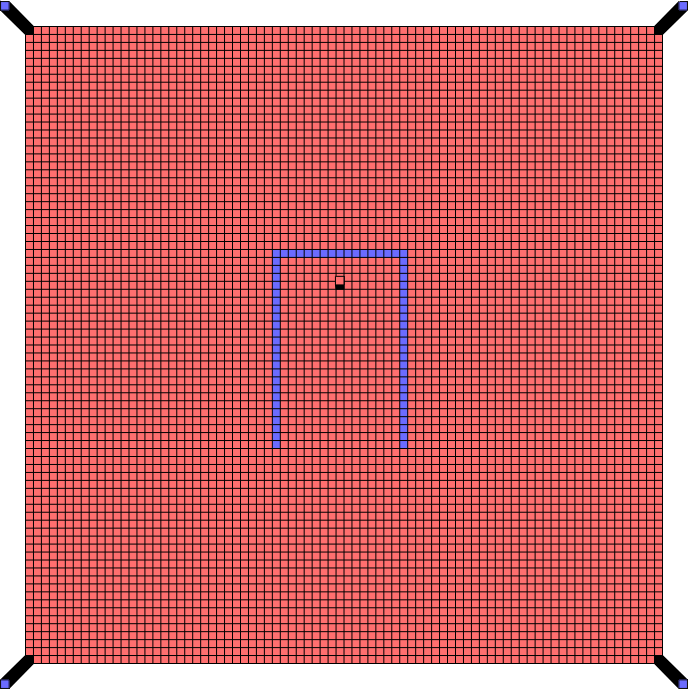
\includegraphics[totalheight=3.in]{figures/PiPermeabilityMapAndWells.png} 
       \end{center}
     \caption{Injection wells (blue) and production well (red) for Example~1. Background shows $\tens{k}_x$ ($ \tens{k}_x = \tens{k}_y$).}
  \label{fig:PImodelPermeabilityMapAndWells}
\end{figure}



\begin{table}
\centering
\caption{Oil production in $10^3$~m$^3$ (Example 1, {\bf 40 control variables}) for the optimized objective function
         without satisfying the nonlinear constraints (`Unconstr.'), satisfying the nonlinear constraints
         using the heuristic treatment (`Heuristic'), and satisfying the nonlinear constraints
         using the formal approach (`Formal'). Best feasible results shown in bold.}
\begin{tabular}{|c|c|c|c|}
\hline
   Run & Unconstr. & Heuristic & Formal                       \\
\hline
Reference    & 163.9         &  152.2                      &                           \\
1                     & 187.5         &  156.6                      &        158.2        \\
2                     & 189.1         &  162.0                      &        146.2        \\
3                     & 177.3         &  149.0                      &        149.2        \\
4                     & 183.4         &  150.2                      & \bf{ 160.6 }      \\
5                     & 186.1         &  152.2                      &        152.9        \\
6                     & 185.0         &  158.9                      &        160.2        \\
7                     & 190.2         &  162.3                      &        142.5        \\ 
8                     & 190.1         &\bf{163.5}                 &        158.5        \\
9                     & 190.1         &     162.0                   &        158.0        \\
\hline
\end{tabular}
  \label{table:PiC500Steps8}
\end{table}


   
          
             
\begin{table}
\centering
\caption{Oil production in $10^3$~m$^3$ (Example 1, {\bf 320 control variables}) for the optimized objective function
         without satisfying the nonlinear constraints (`Unconstr.'), satisfying the nonlinear constraints
         using the heuristic treatment (`Heuristic'), and satisfying the nonlinear constraints
         using the formal approach (`Formal'). Best feasible results shown in bold.}
\begin{tabular}{|c|c|c|c|}
\hline
   Run & Unconstr. & Heuristic & Formal                          \\
\hline
Reference             & 150.1         &  152.5                      &                     \\
1                     & 188.1         &  149.9                      &  \bf{ 170.2 }        \\
2                     & 192.4         &  155.6                      &         131.4            \\
3                     & 186.5         &  136.4                      &         117.8          \\
4                     & 186.8         &  149.9                      &         133.7          \\
5                     & 186.5         &  142.2                      &         156.1          \\
6                     & 192.5         &  157.8                      &         168.2          \\
7                     & 192.5         &  \bf{159.4}               &         158.8          \\ 
8                     & 192.4         &  156.9                      &         161.1          \\
9                     & 192.2         &  157.0                      &         165.8          \\
\hline
\end{tabular}
  \label{table:PiC500Steps64}
\end{table}
 
 
 
 

 



%\begin{figure}[htb]
%\begin{center}
%     \begin{tabular}{ccccccccc}
%      0 &  0.125 & 0.250 & 0.375 & 0.500 & 0.625 & 0.750 & 0.875 & 1
%      \end{tabular}
%      
\includegraphics[width=8cm, height=0.5cm]{VanEssenModelPermeabilityMapColorBar.png}
%       
%       \medskip
%
%       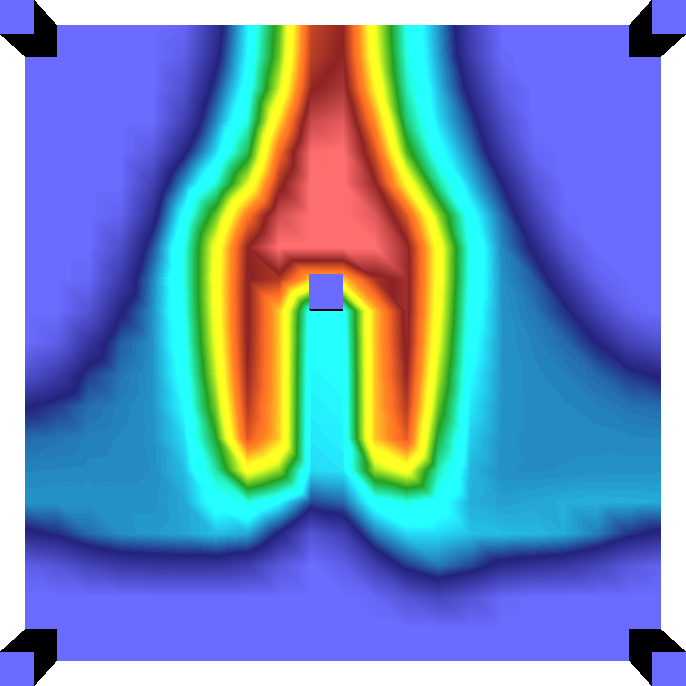
\includegraphics[totalheight=3.in]{PiBenchmarkSteps256RefenceC500T256.png} 
%
%       \medskip
%
%       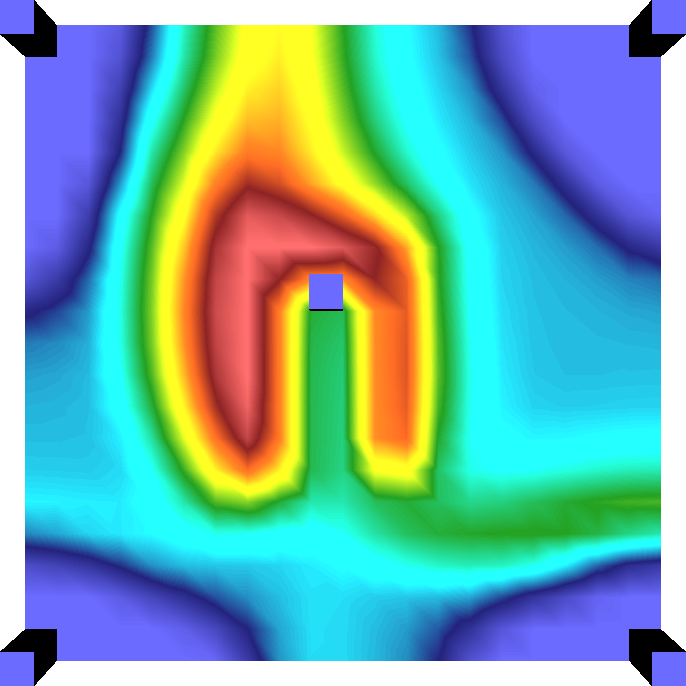
\includegraphics[totalheight=3.in]{PiBenchmarkSteps256HeuristicC500T256.png} 
%
%       \medskip
%
%       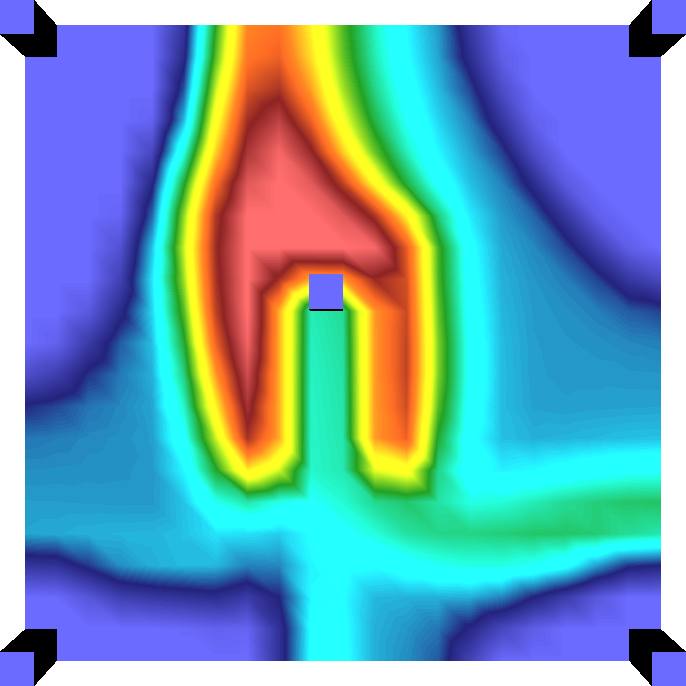
\includegraphics[totalheight=3.in]{PiBenchmarkSteps256FormalC500T256.png} 
%
%       \end{center}
%     \caption{Injection wells (blue) and production wells (red) for Example 1. Background shows $\tens{K}_x$ ($ \tens{K}_x = \tens{K}_y$).}
%  \label{fig:PImodelOilSaturation}
%\end{figure}

\begin{figure} [ht]
\begin{center}
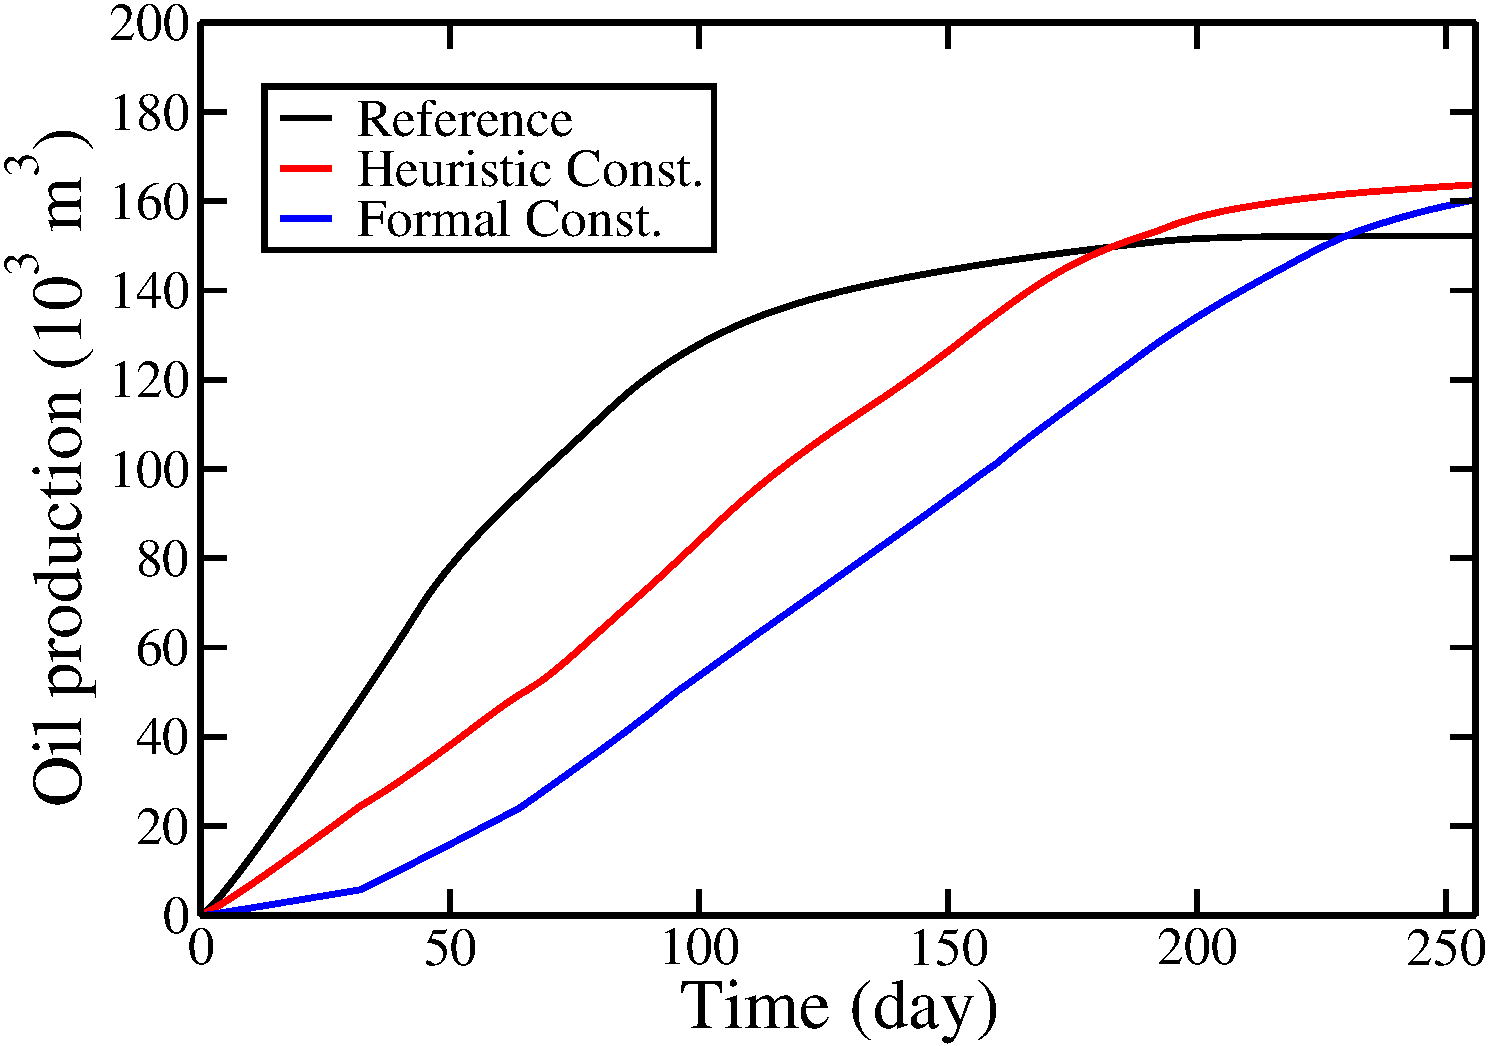
\includegraphics[totalheight=2.17in,angle=0]{figures/RevenuePI2.pdf}
\end{center}
\caption{Oil production versus time (Example 1, 40 control variables). Results are for
  feasible reference case (black curve), best heuristically constrained solution (Run 8, red curve)
  and best formally constrained solution (Run 4, blue curve).}
\label{fig:PIRevenue}
\end{figure}
\begin{figure}
\begin{center}
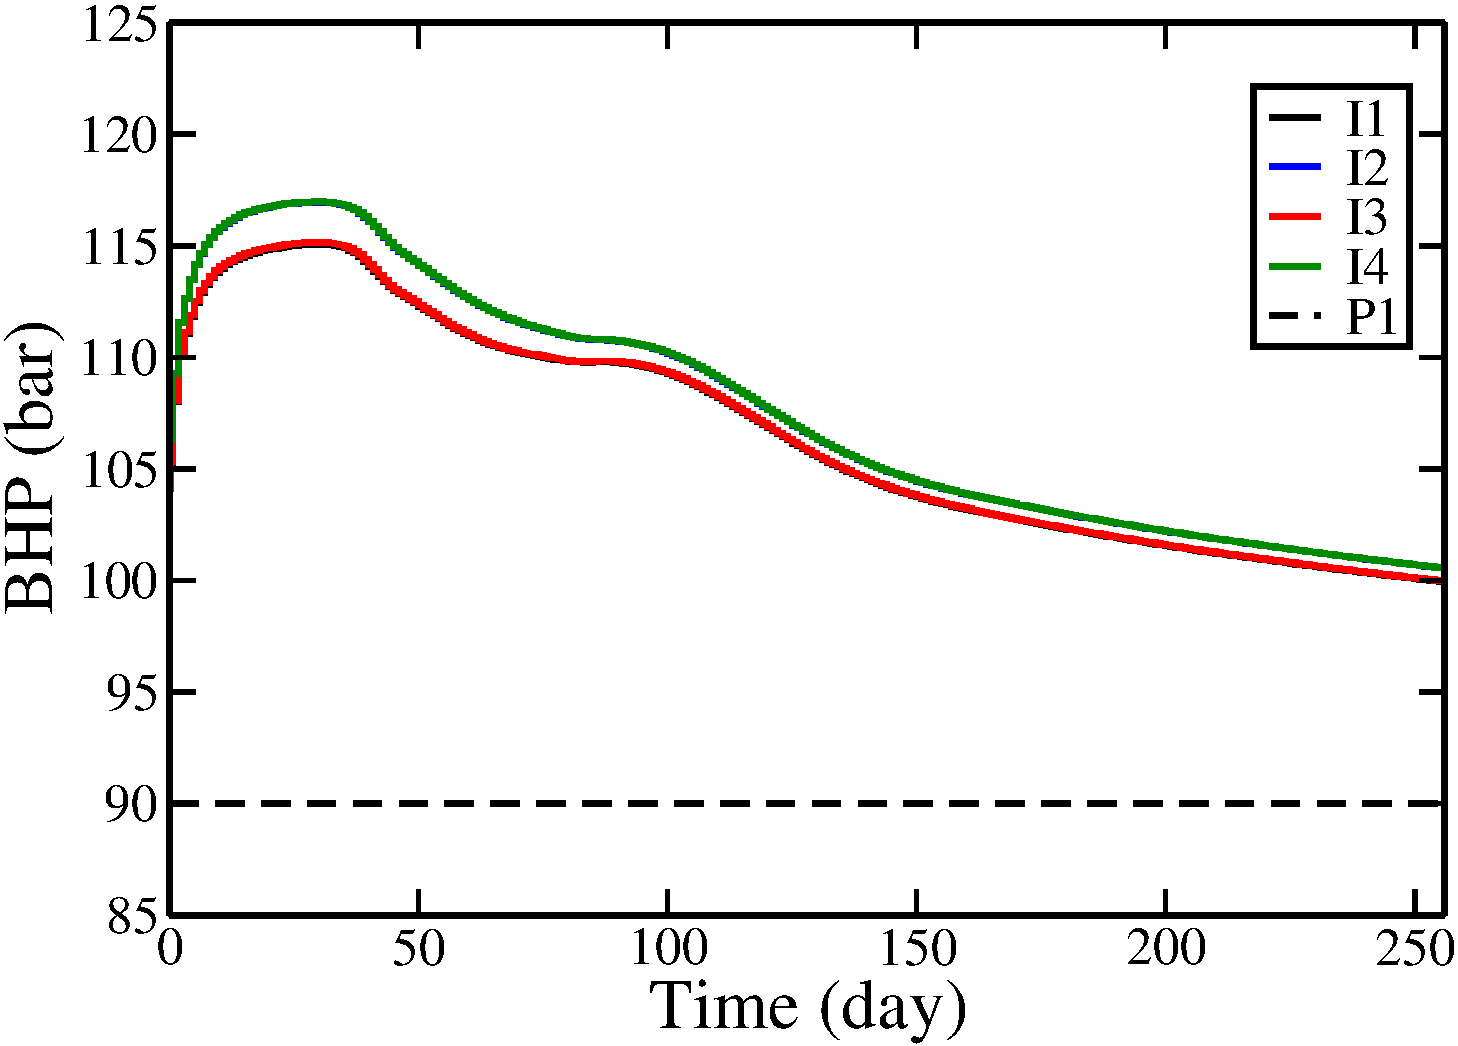
\includegraphics[totalheight=2.2in,angle=0]{figures/ReferenceC500HeuristicItPb_BHP.pdf}
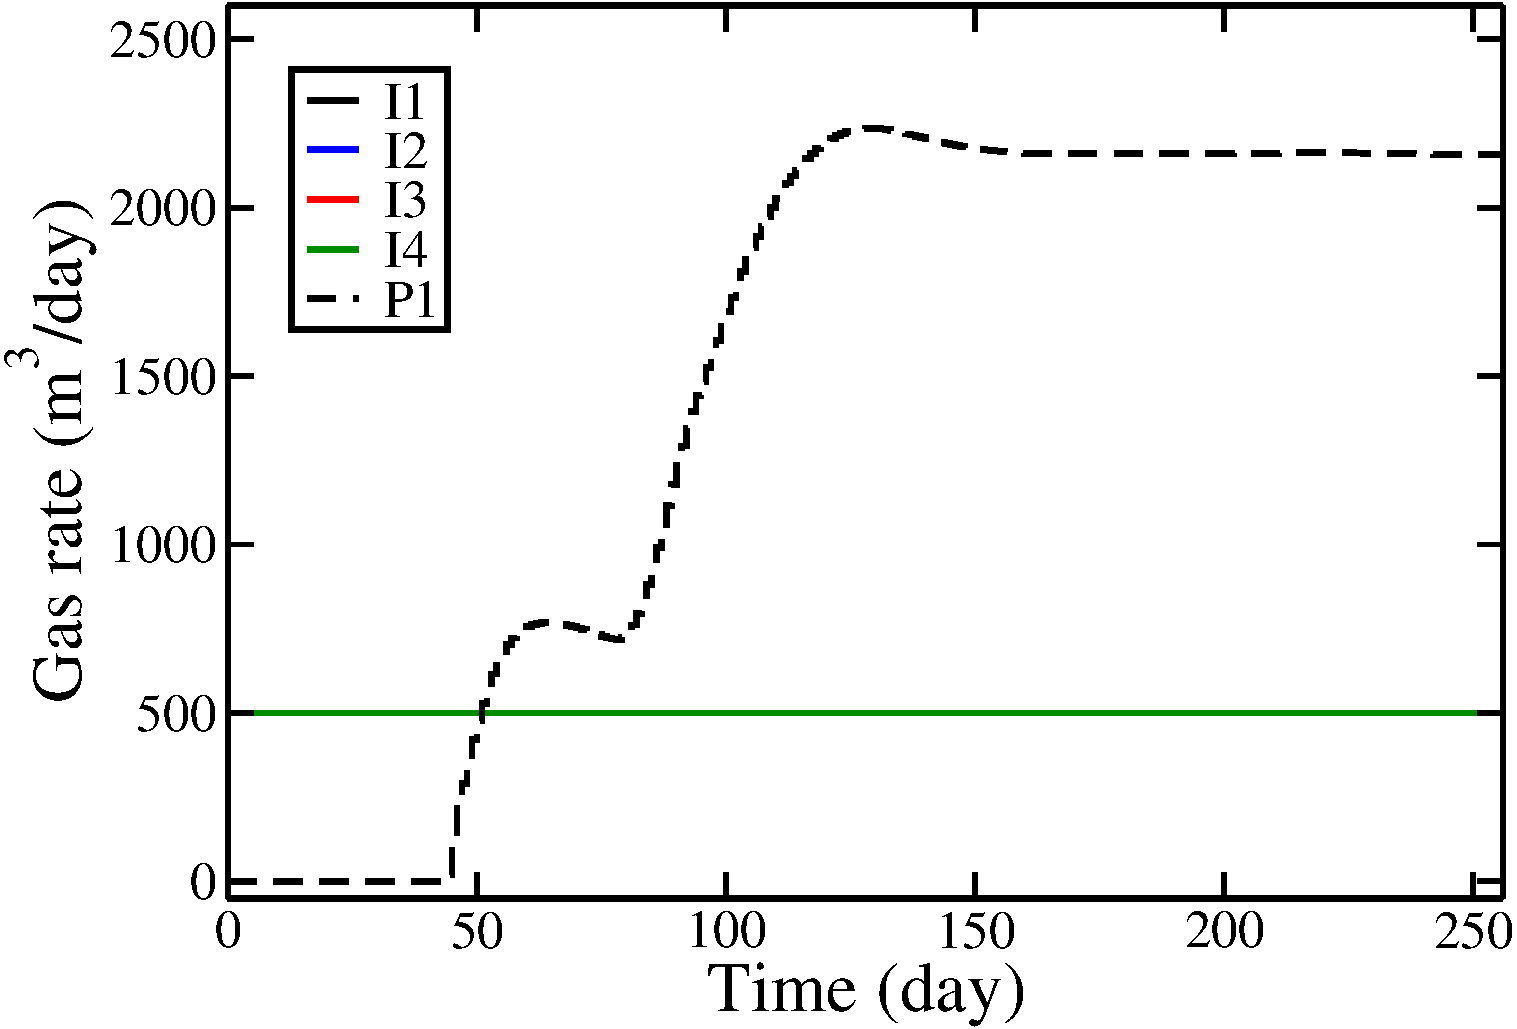
\includegraphics[totalheight=2.17in,angle=0]{figures/ReferenceC500HeuristicItPb_rate_gas.pdf}
\end{center}
\caption{BHPs (top) and gas rates (bottom) for the feasible reference solution (Example 1). 
  Gas injection rates are all equal to 500~m$^3$/d during the entire simulation period. }
\label{fig:PIReferencePlots}
\end{figure}




%%%%%%%%%%%%%%%%%%%%%%%%%%% Pi 40 controls    %%%%%%%%%%%%%%%%%%%%%%%%%%%%%%

\begin{figure}
\begin{center}
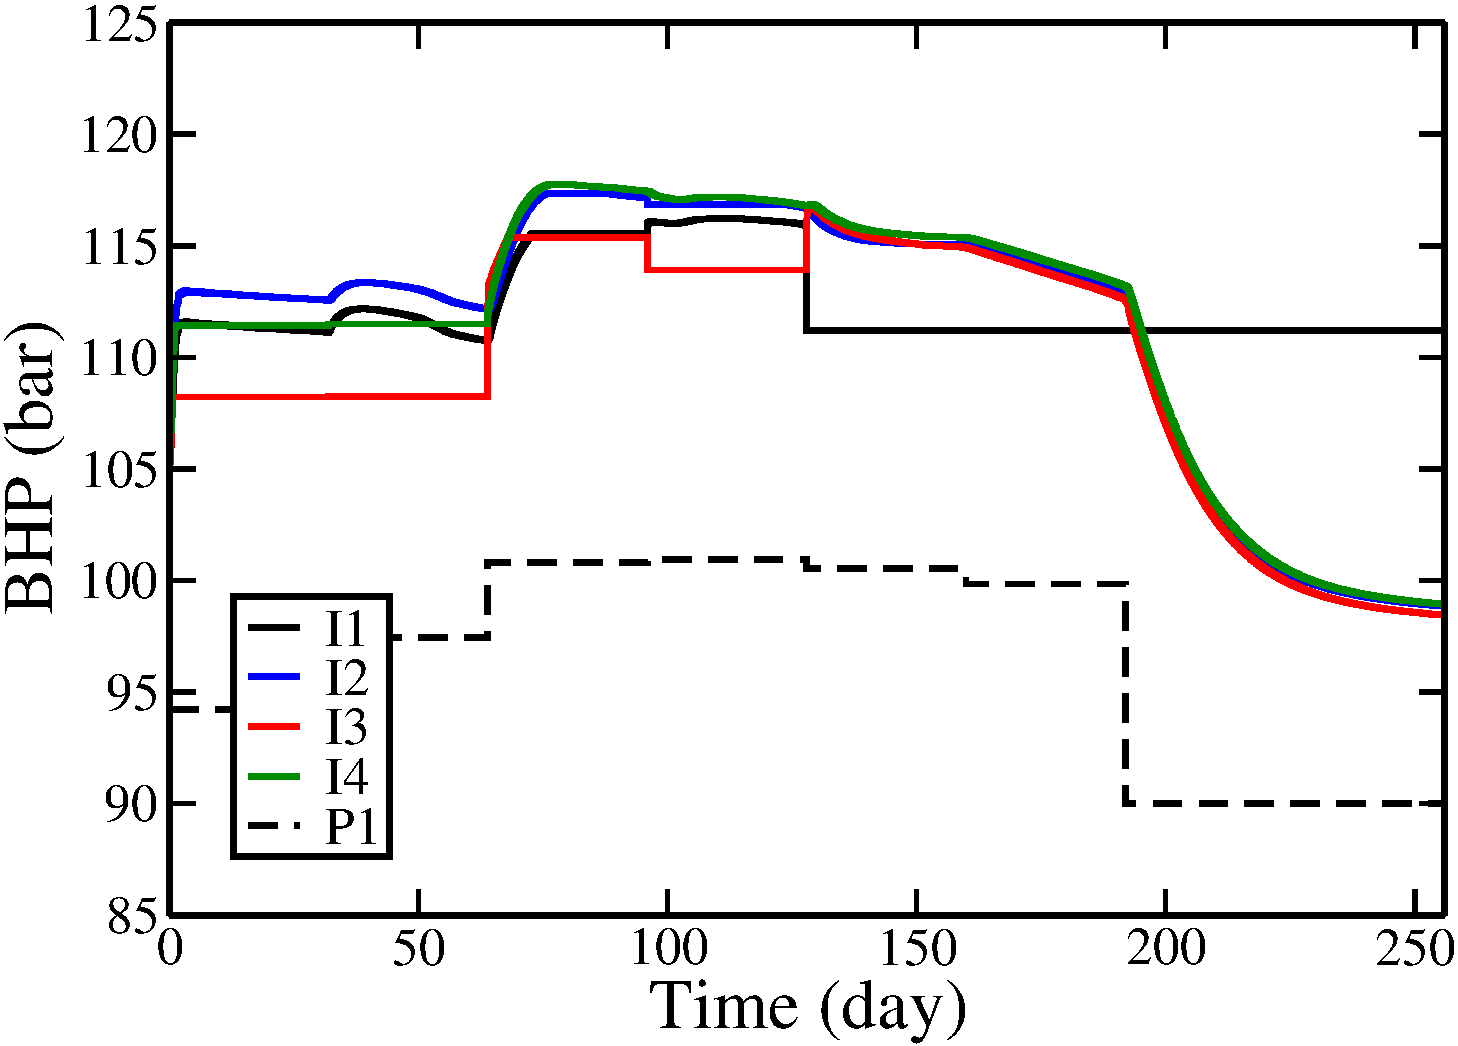
\includegraphics[totalheight=2.2in,angle=0]{figures/HeuristicC500Steps8OptimalItPm_BHP.pdf}
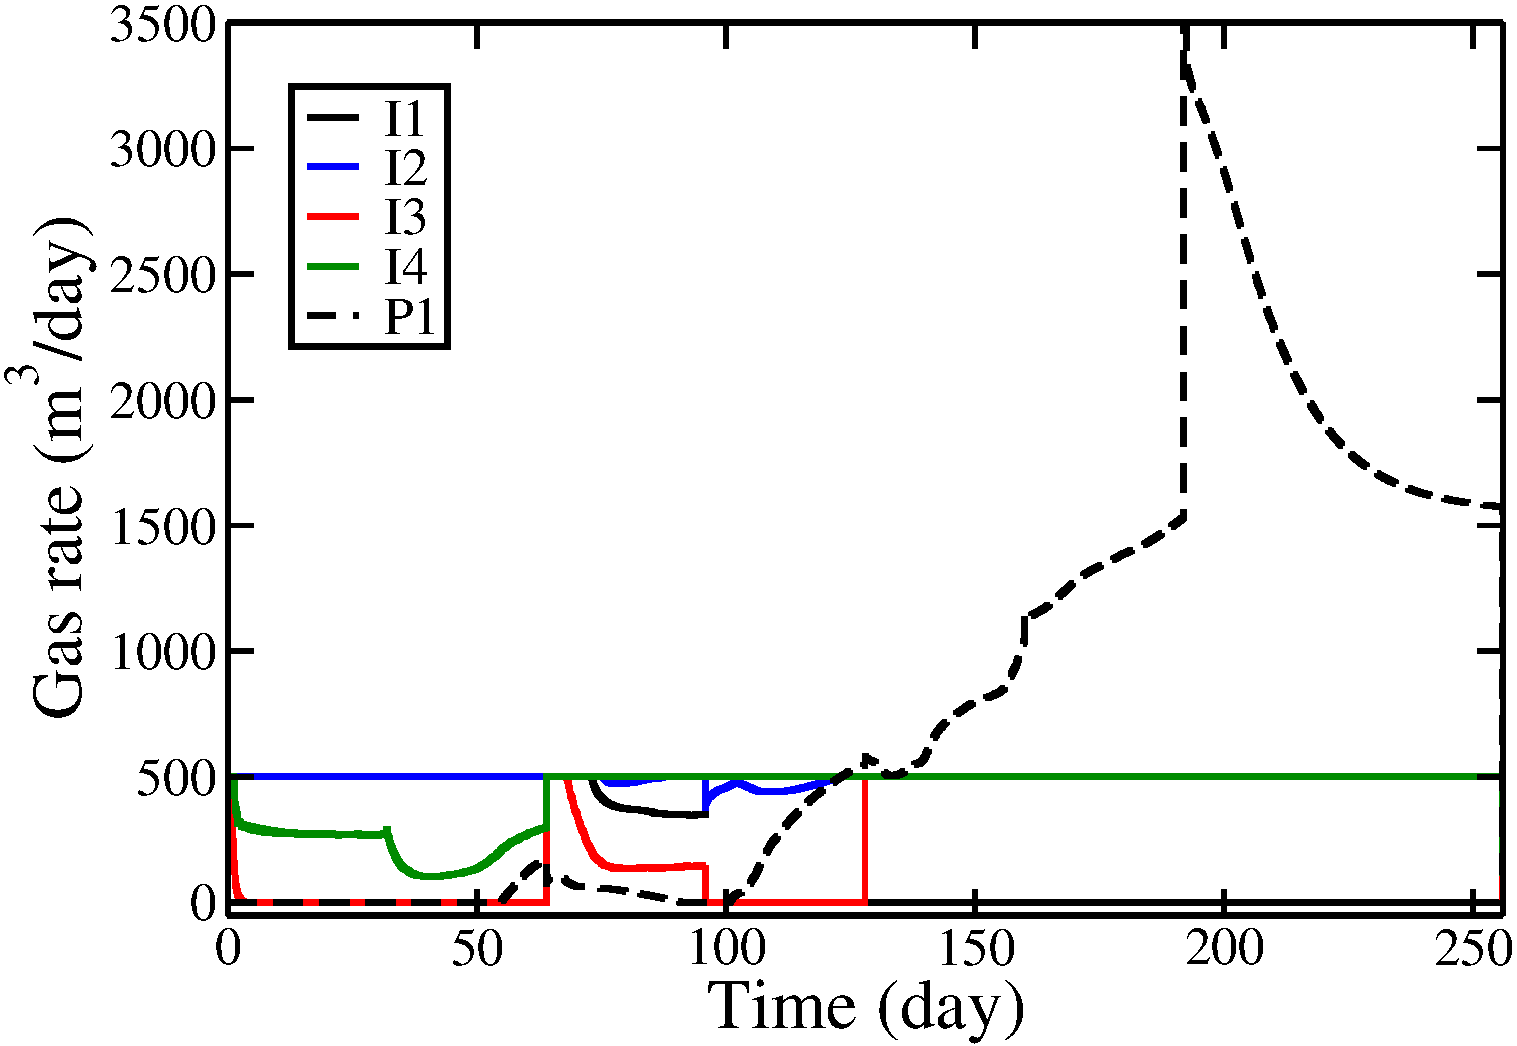
\includegraphics[totalheight=2.17in,angle=0]{figures/HeuristicC500Steps8OptimalItPm_rate_gas.pdf}
\end{center}
\caption{BHPs (top) and gas rates (bottom) for the best heuristically constrained solution using 40 controls (Example 1, Run 8).}
\label{fig:PIHeuristicControls40Plots}
\end{figure}

\begin{figure}
\begin{center}
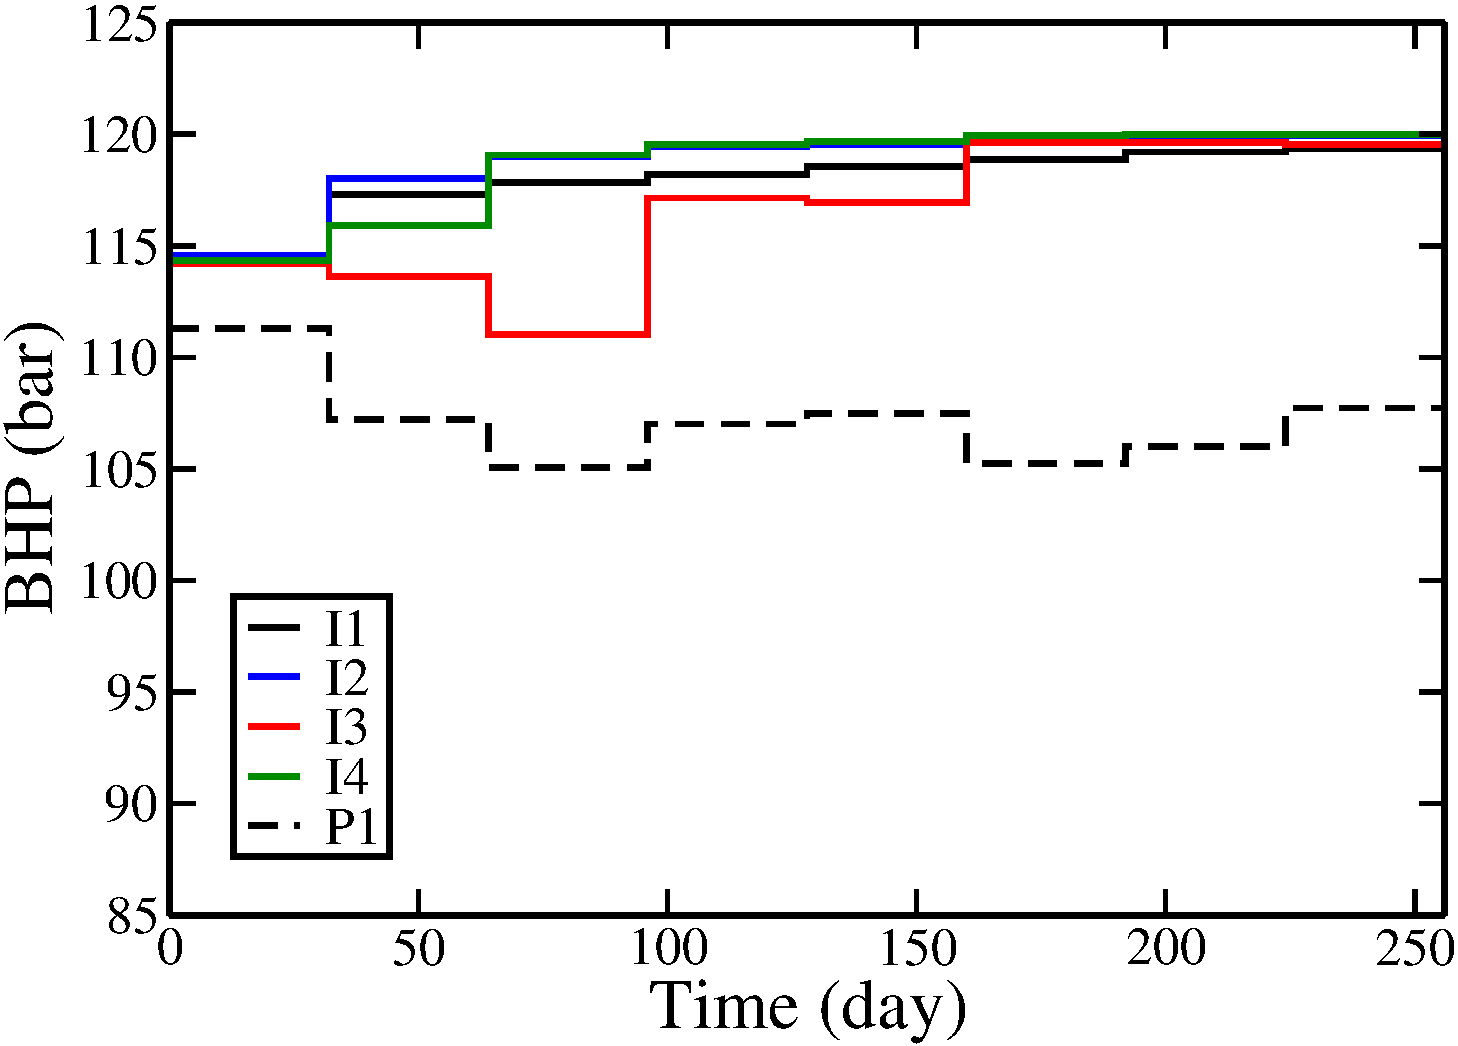
\includegraphics[totalheight=2.2in,angle=0]{figures/FormalC550Steps8OptimalImPb_BHP.pdf}
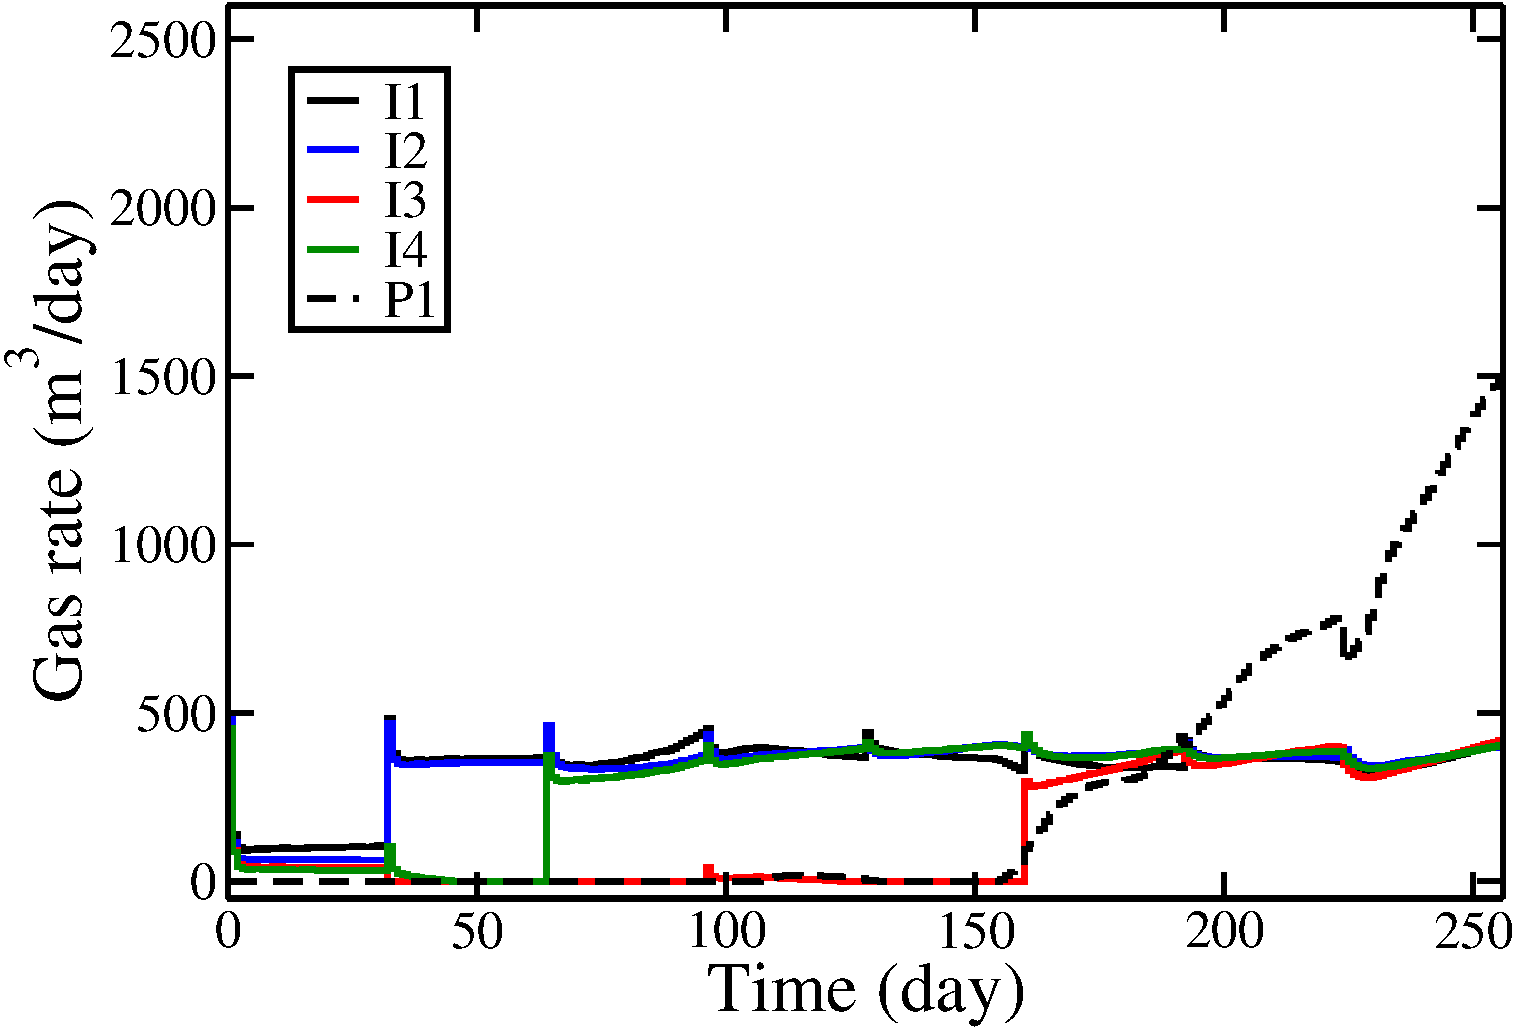
\includegraphics[totalheight=2.17in,angle=0]{figures/FormalC550Steps8OptimalImPb_rate_gas.pdf}
\end{center}
\caption{BHPs (top) and gas rates (bottom) for the best formally constrained solution using 40 controls (Example 1, Run 4).}
\label{fig:PIFormalControls40Plots}
\end{figure}




\begin{figure}
\begin{center}
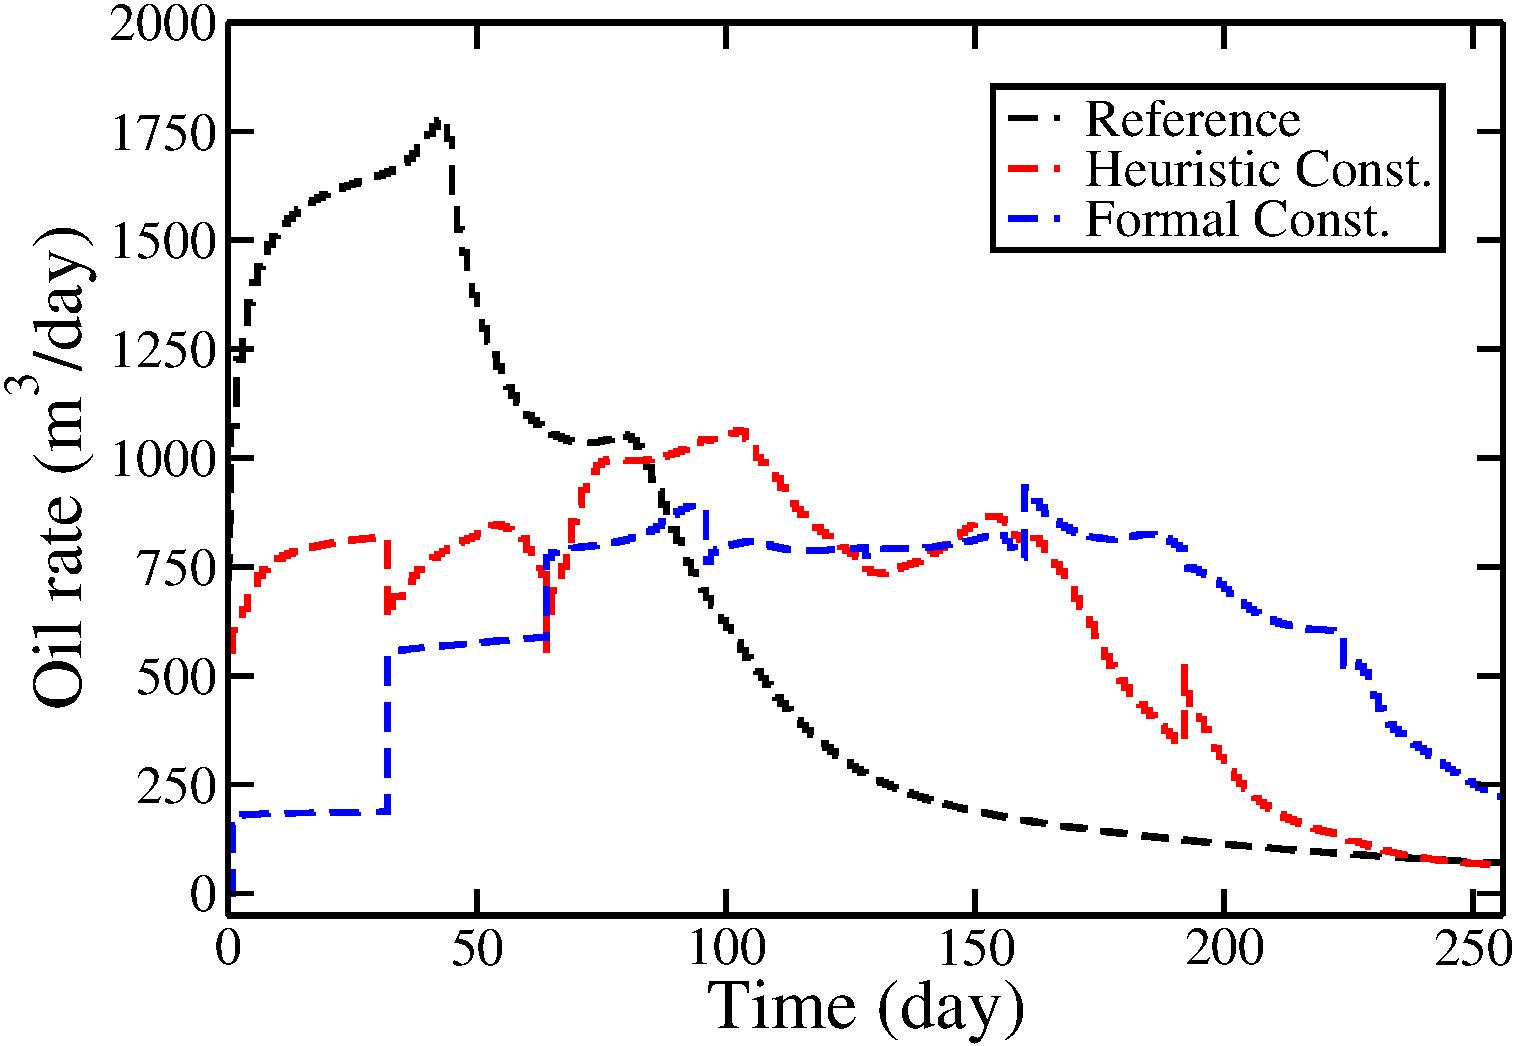
\includegraphics[totalheight=2.2in,angle=0]{figures/OilRatesSteps8.pdf}
%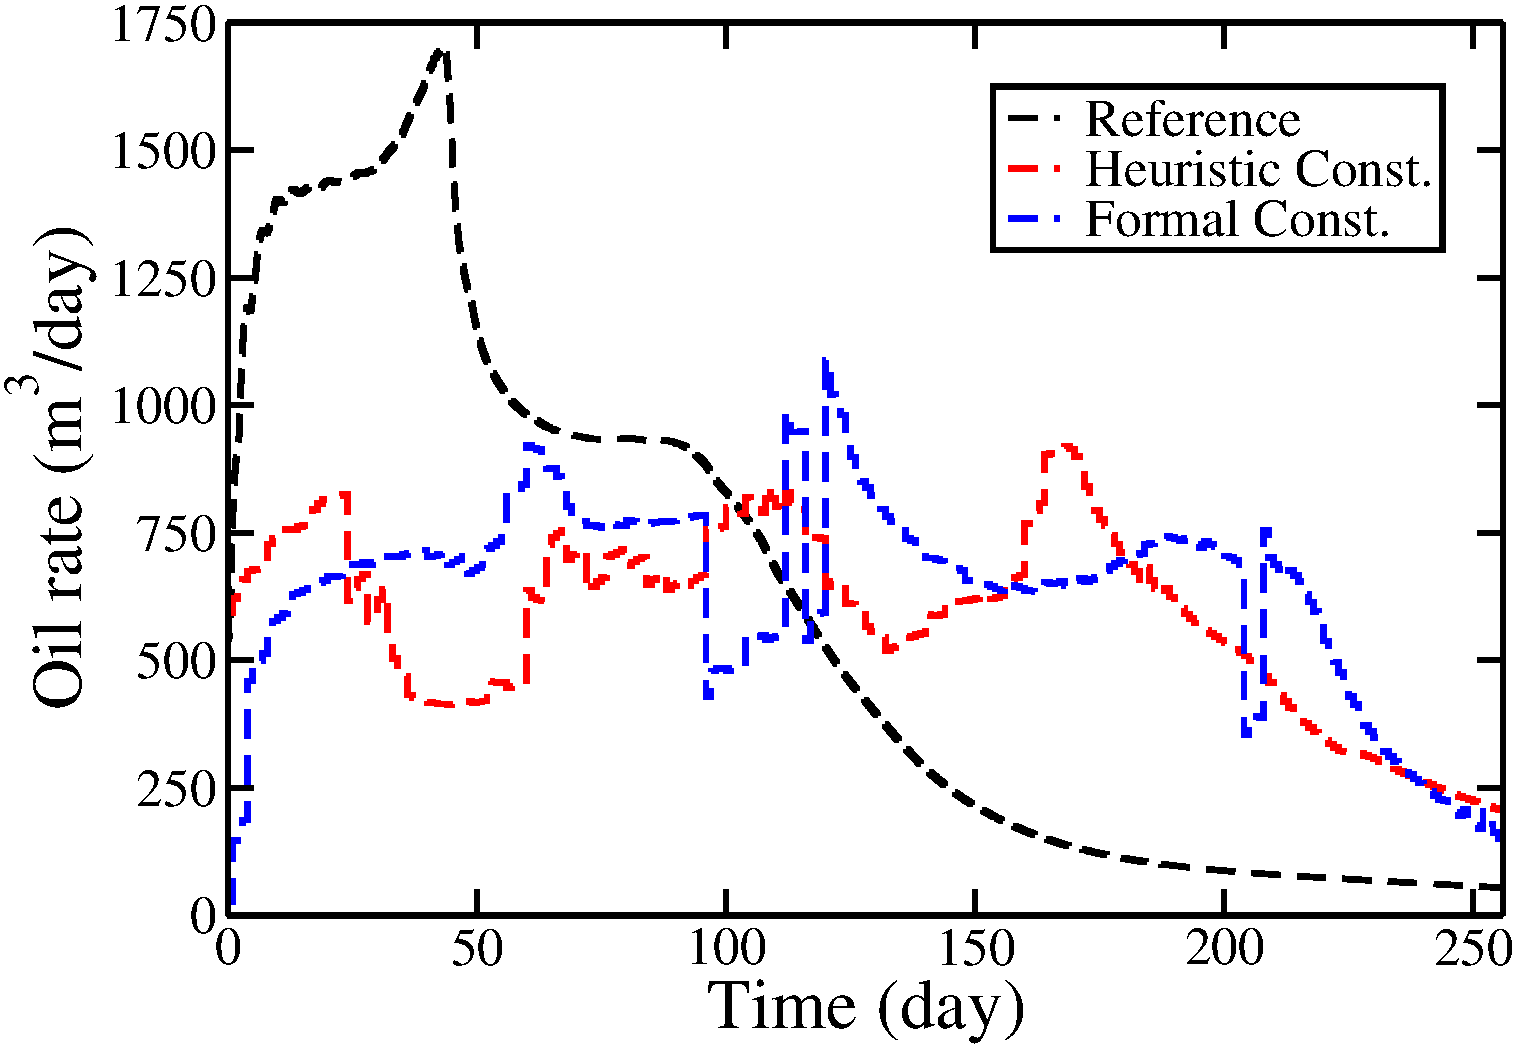
\includegraphics[totalheight=2.2in,angle=0]{OilRatesSteps64.pdf}
%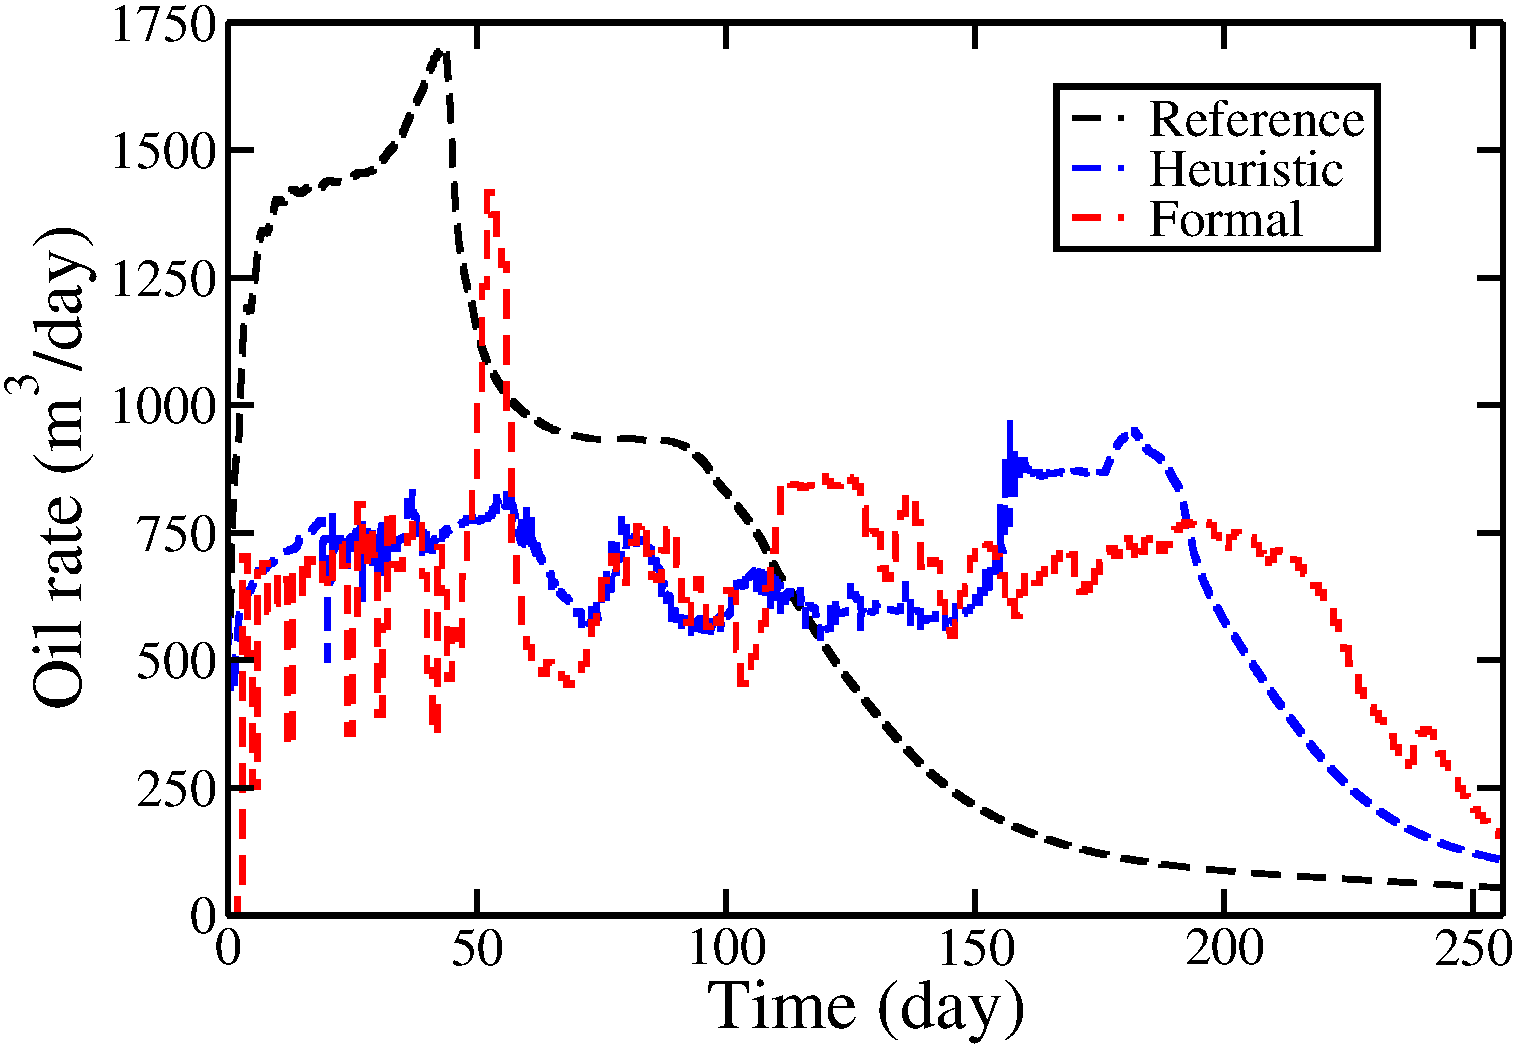
\includegraphics[totalheight=2.2in,angle=0]{OilRates.pdf}
\end{center}
\caption{Oil rates for Example 1 (40 controls), reference (black dashed line), heuristically constrained (red dashed line)
 and formally constrained (blue dashed line).} 
\label{fig:PIOilRates}
\end{figure}





\subsection{Example 2 - Top layer of SPE 10 model}
%
In the second example we again maximize cumulative oil recovery under CO$_2$
injection. The two-dimensional geological model is the top layer of the model
defined in the SPE comparative solution project~\cite{Christie}, referred to as
SPE~10. The model includes a total of four components, as specified in
Table~\ref{table:fluidForSPE10TopLayer}. Details on the
reservoir model are provided in
Table~\ref{table:spe10toplayer}.

%
\begin{table}
\centering
\caption{Fluid description for Example 2}
\begin{tabular}{|l|r|r|r|r|}
\hline
%\multicolumn{5}{|c|}{SPE10 top layer}    \\
%\hline
Component            & CO$_2$ & C$_1$ & C$_4$ & C$_{10}$    \\
\hline
Initial composition (\%)  & 1    & 20  & 29    & 50 \\
Injection composition (\%)& 90   & 10 & - & - \\
\hline
\end{tabular}
\label{table:fluidForSPE10TopLayer}
\end{table}
%


\begin{table}
\centering
\caption{Model parameters for Example 2}
\begin{tabular}{|l|rr|}
\hline
%\multicolumn{3}{|c|}{SPE10 top layer}  \\
%\hline
Grid size                & 60 $\times$ 220 $\times$ 1 &       \\
\hline\hline
Parameter                & Value    & Units \\
\hline
$\Delta x$               & 6.096&m          \\
$\Delta y$               & 3.048&m          \\
$\Delta z$               & 0.6096&m         \\
Depth                    & 2574&m           \\
Initial pressure         & 75  & bar        \\
Temperature              &$100$ & $^\circ$C     \\
\hline
Rock compressibility     & $7.2 \times 10^{-5}$ & 1 / bar \\
Simulation time          &1000 & d          \\
Pressure upper bound     & 150 & bar        \\
Pressure lower bound     &  50 & bar        \\
\hline
Residual gas saturation  & 0 & -            \\
Residual oil saturation  & 0 & -            \\
End point rel perm gas   & 1 & -            \\
End point rel perm oil   & 1 & -            \\
Corey exponent gas       & 2 & -            \\
Corey exponent oil       & 2 & -            \\
\hline\hline
Well locations [grid block no.] & $i$ & $j$     \\
\hline
Injector 1               &   58&   9   \\
Injector 2               &   58& 126   \\
Injector 3               &    2&  67   \\
Injector 4               &    2& 211   \\
Producer 1               &    2&   3   \\
Producer 2               &   58&  67   \\
Producer 3               &    2& 143   \\
Producer 4               &   58& 210   \\
\hline
\end{tabular}
\label{table:spe10toplayer}
\end{table}



The well locations, along with a map of the permeability field, are depicted in
Fig.~\ref{fig:PermeabilityMapAndWellsSpe10Top}. The control parameters in the
optimization problem are again well BHPs, constrained to lie between 150~bar and 50~bar. A
maximum (per well) gas production rate of 200~m$^3/$d at reservoir conditions is also specified.
The total simulation period is 1000~days. The well controls are determined
at initial time and then at every 100-day interval. There are a
total of ten control steps and 80 control parameters in this example.


%
\begin{figure}[ht]
\begin{center}
     \begin{tabular}{cccccccc}
      0.003 &  0.023 & 0.178 & 1.358 & 10.38 & 79.43 & 607.6 &4648
      \end{tabular}
      
\includegraphics[width=8cm, height=0.5cm]{figures/VanEssenModelPermeabilityMapColorBar.png}
       
       \medskip

       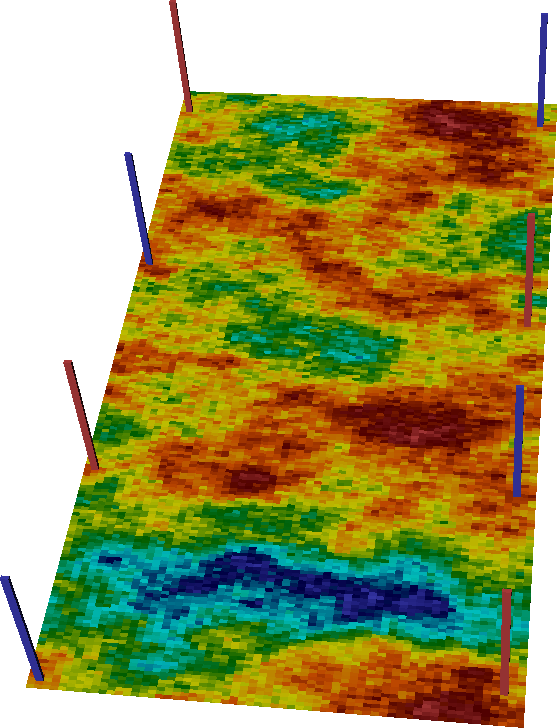
\includegraphics[totalheight=3.2in]{figures/SPE10TopModelPermeabilityMapConstantRotated.png} %SPE10TopPermeabilityMapAndWells.png}

        %\medskip

       %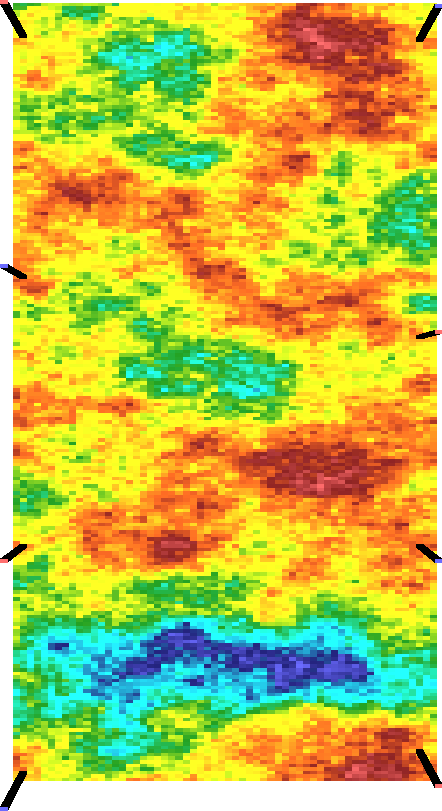
\includegraphics[totalheight=3.2in, angle=270]{SPE10TopModelPermeabilityMapConstant.png} %SPE10TopPermeabilityMapAndWells.png}
\end{center}
     \caption{Injection wells (blue) and production wells (red) for Example~2. Background shows $\log \tens{k}_x$ ($\tens{k}_x = \tens{k}_y$).}
  \label{fig:PermeabilityMapAndWellsSpe10Top}
\end{figure}
%

\begin{table}
\centering
\caption{Oil production in $10^3$~m$^3$ (Example 2) for the optimized objective function
         without satisfying the nonlinear constraints (`Unconstr.'), satisfying the nonlinear constraints
         using the heuristic treatment (`Heuristic'), and satisfying the nonlinear constraints
         using the formal approach (`Formal'). Best feasible results shown in bold.}
\begin{tabular}{|c|c|c|c|}
\hline
  Run            &  Unconstr. & Heuristic & Formal      \\
\hline
Reference        & 20.29         &     20.28         & 	         \\
1 & 21.77      &     21.77         &       21.77    \\
2 & 22.01      &     22.01         &       22.01    \\
3 & 18.16      &     18.16         &       18.17    \\
4 & 21.68      &     21.68         &       21.68    \\
5 & 22.03      & \bf{22.03}      &       22.04    \\
6 & 22.13      &     20.67         &  \bf{22.20}    \\
7 & 21.68      &     21.68         &       21.99    \\
8 & 22.07      &     21.48         &       22.07    \\
9 & 22.03      & \bf{22.03}      &       22.03    \\
\hline
\end{tabular}
  \label{table:spe10top}
\end{table}

%1 & O25G16     &     21400         &       O78G57 \\
%2 & O25G16     & \bf{21980}        &       O46G35 \\
%3 & O48G34     &     16800         &       O31G22 \\
%4 & O25G17     &     21600         &       O79G46 \\
%5 & O21G17     &     19900         &       O140G62\\
%6 & O28G15     &     19800         &       O41G32 \\
%7 & O24G15     &     21000         &       O77G61 \\
%8 & O21G14     &     20500         &       O67G49 \\
%9 & O29G19     &     20900         &       O77G49 \\


We first generate two reference solutions as in the previous example. The cumulative oil production for these two cases, given in the first row (`Reference') of Table~\ref{table:spe10top}, are nearly identical because the nonlinear constraint violation in the
unconstrained case is small. We next perform (nine) optimizations that honor the bound constraints but not the nonlinear constraints. The best optimum achieved in this case provides a cumulative oil production of 22,130~m$^3$ (Run~6). Using the heuristic constraint handling procedure (third column), the best result is 22,030~m$^3$ of oil (Runs~5 and 9), which
exceeds the reference heuristic result by 8.8\%. The best optimum achieved using the formal constraint handling treatment is 22,200~m$^3$ of oil (Run~6). This value exceeds the reference solution by 9.5\% and the best result using the heuristic treatment by 0.8\%. It also exceeds the best unconstrained result (again, unconstrained here refers to the nonlinear constraints) of 22,130~m$^3$, which is presumably because the nonlinear constraints are not very important in this example.

Oil production profiles are shown in Fig.~\ref{fig:SPE10TopLayerRevenue}. These profiles are very similar for the runs using the heuristic and formal constraint handling procedures. The BHP, gas rate, and oil rate profiles for the three cases are shown in
Figs.~\ref{fig:SPE10TopLayerReferenceRates},
\ref{fig:SPE10TopLayerUnconstrainedOptimalChoppedRates} and
\ref{fig:SPE10TopLayerConstrainedOptimalRates}. We see that the gas production rates satisfy the nonlinear constraints (200~m$^3/$d) at all times for both constraint handling procedures. Consistent with Fig.~\ref{fig:SPE10TopLayerRevenue}, the oil production rates in Figs.~\ref{fig:SPE10TopLayerUnconstrainedOptimalChoppedRates} and
\ref{fig:SPE10TopLayerConstrainedOptimalRates} resemble one another, and they are clearly different than the reference solution in Fig.~\ref{fig:SPE10TopLayerReferenceRates}. 
For this example, the formal approach required an average of 56 forward simulations, while the heuristic approach required an average of only 24.


\begin{figure} [ht]
\begin{center}
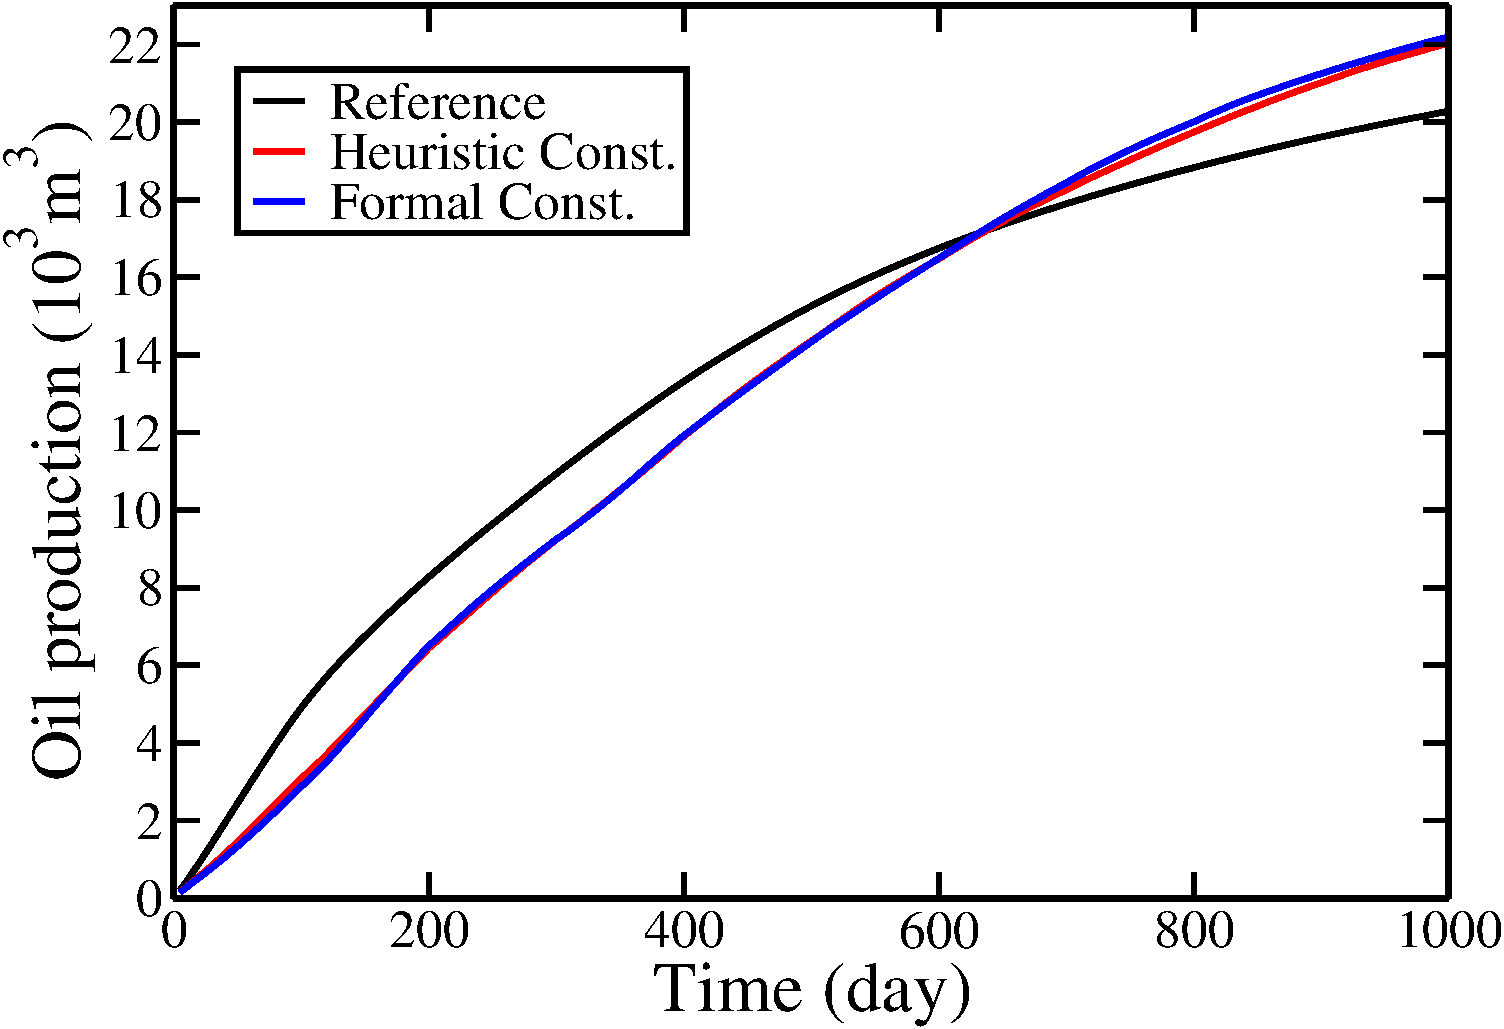
\includegraphics[totalheight=2.17in,angle=0]{figures/spe10TopLayerRevenue.pdf}
\end{center}
\caption{Oil production versus time for Example 2. Results are for
  feasible reference case (black curve), best heuristically constrained solution (Run~9, red curve)
  and best formally constrained solution (Run~6, blue curve).}
\label{fig:SPE10TopLayerRevenue}
\end{figure}
\begin{figure}
\begin{center}
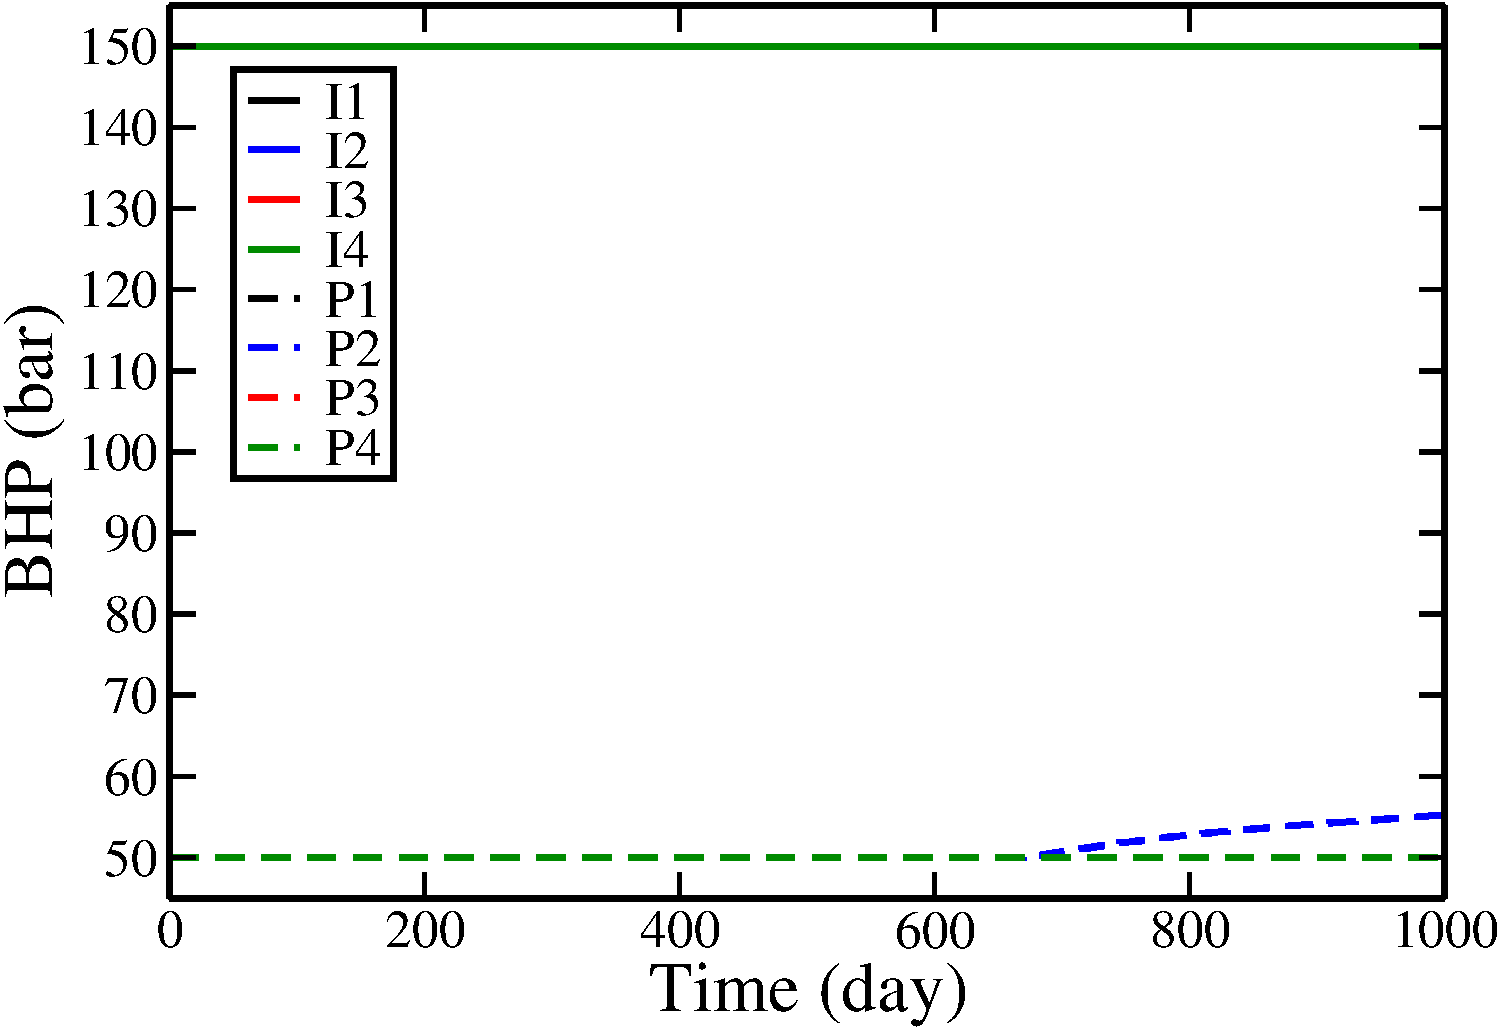
\includegraphics[totalheight=2.2in,angle=0]{figures/spe10topLayerReferenceC200_BHP.pdf}
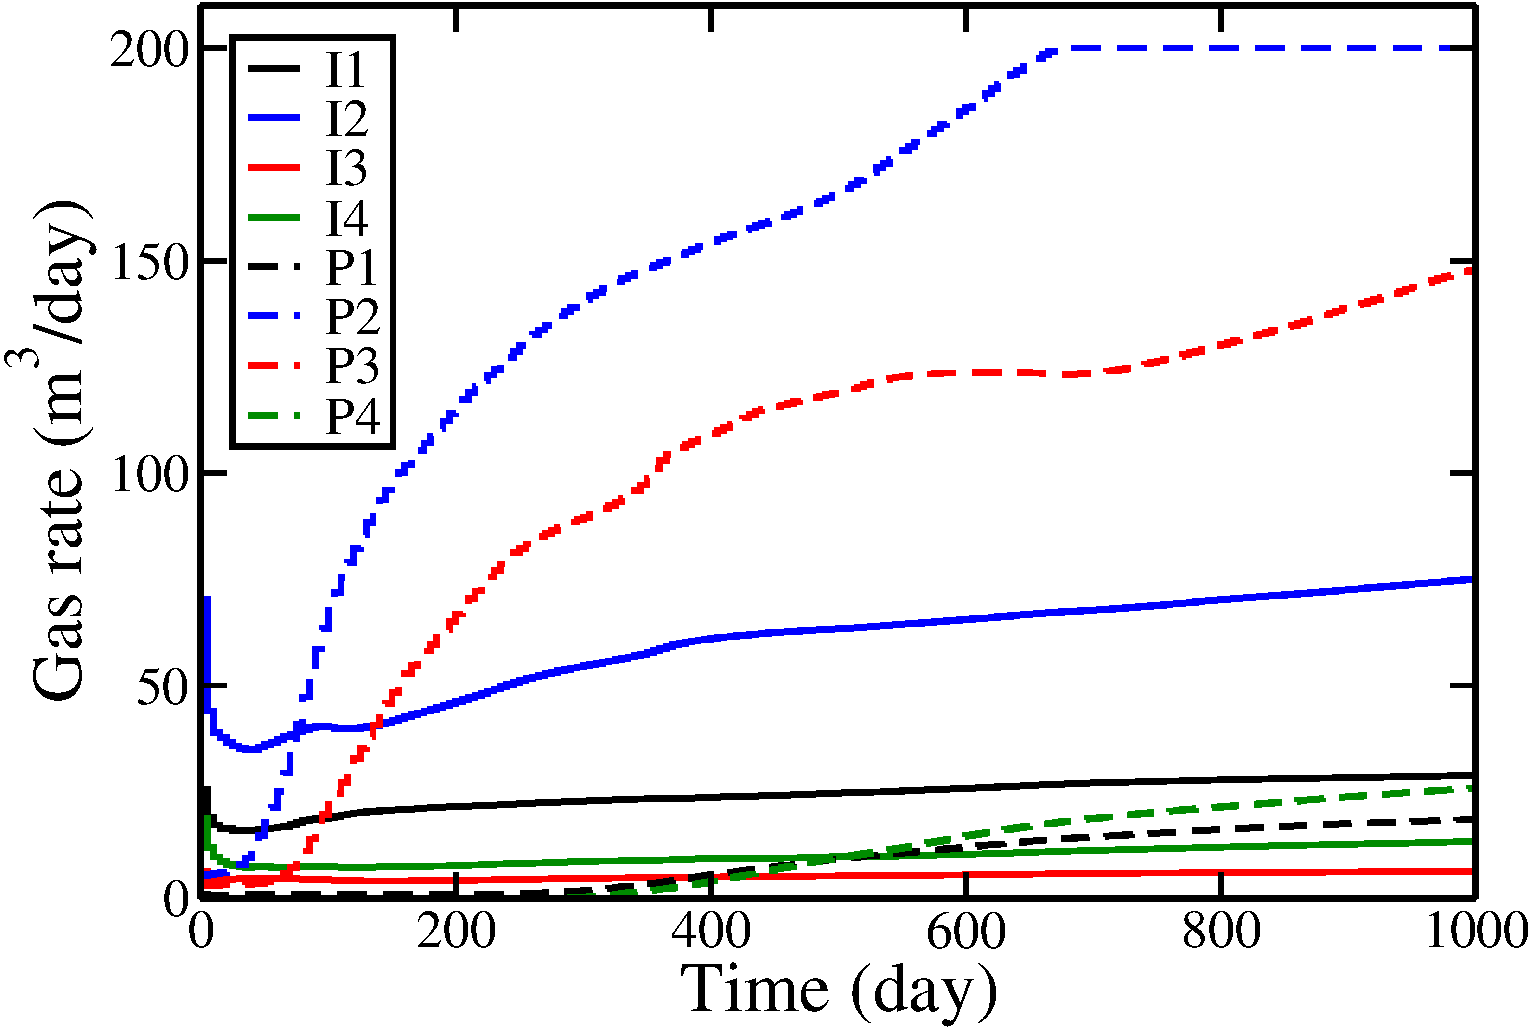
\includegraphics[totalheight=2.17in,angle=0]{figures/spe10topLayerReferenceC200_rate_gas.pdf}
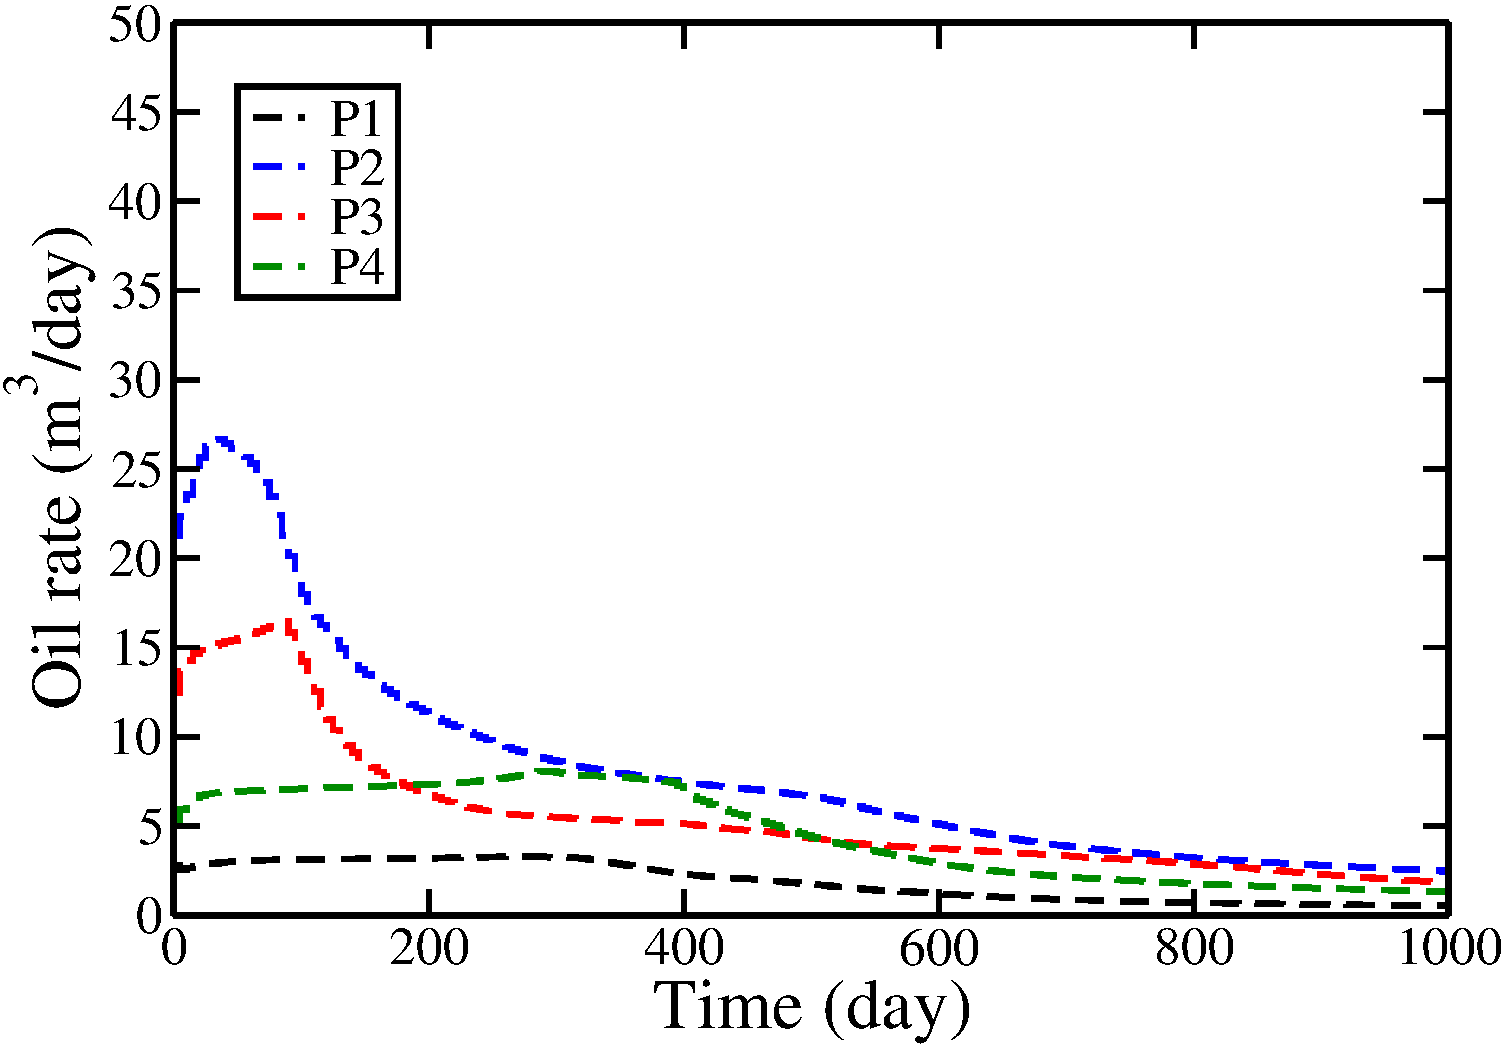
\includegraphics[totalheight=2.2in,angle=0]{figures/spe10topLayerReferenceC200_rate_oil.pdf}
\end{center}
\caption{BHPs (top), gas rates (middle) and oil rates
  (bottom) for the feasible reference solution (Example 2).}
\label{fig:SPE10TopLayerReferenceRates}
\end{figure}

\begin{figure}
\begin{center}
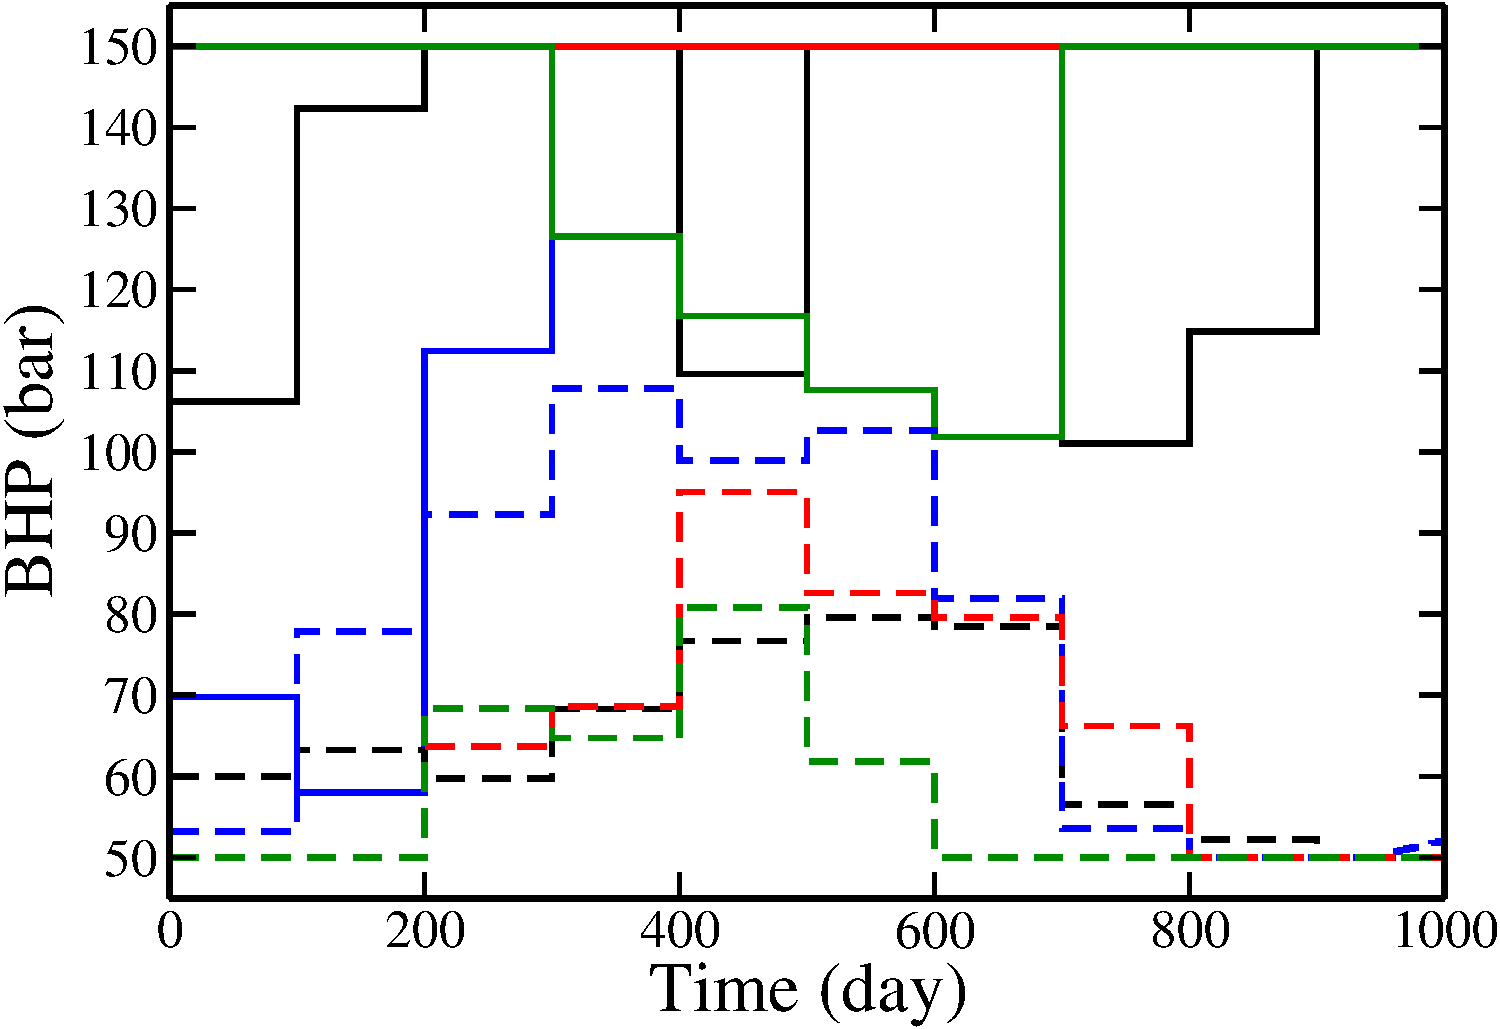
\includegraphics[totalheight=2.2in,angle=0]{figures/spe10topLayerOptimalChoppedIuPu_BHP.pdf}
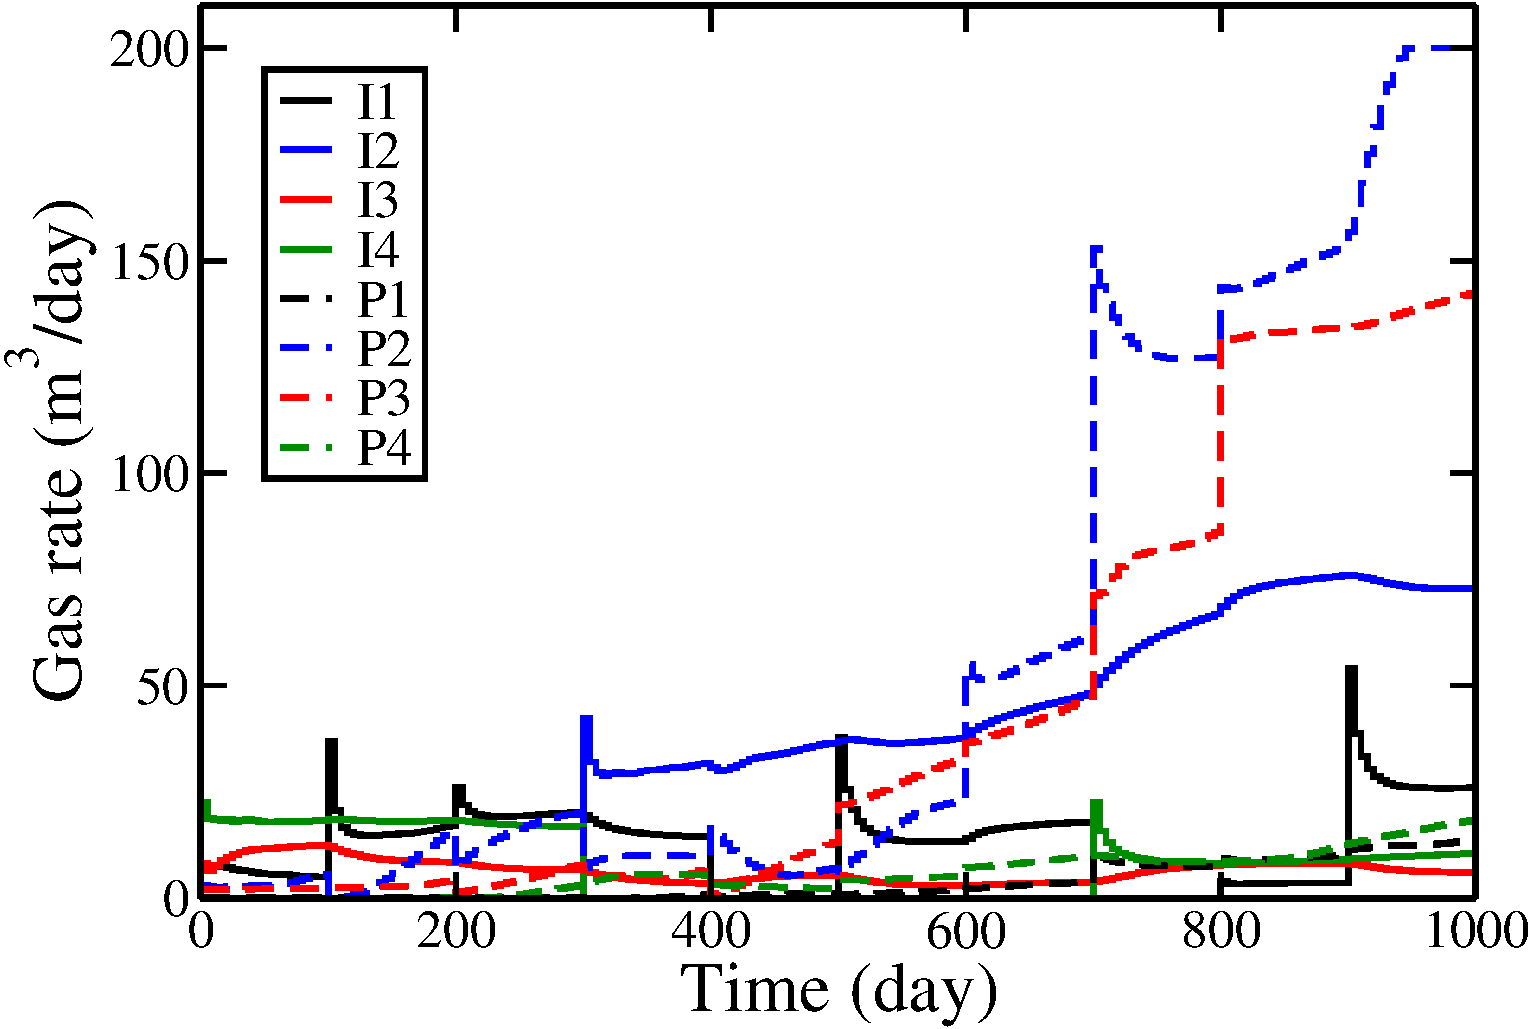
\includegraphics[totalheight=2.17in,angle=0]{figures/spe10topLayerOptimalChoppedIuPu_rate_gas.pdf}
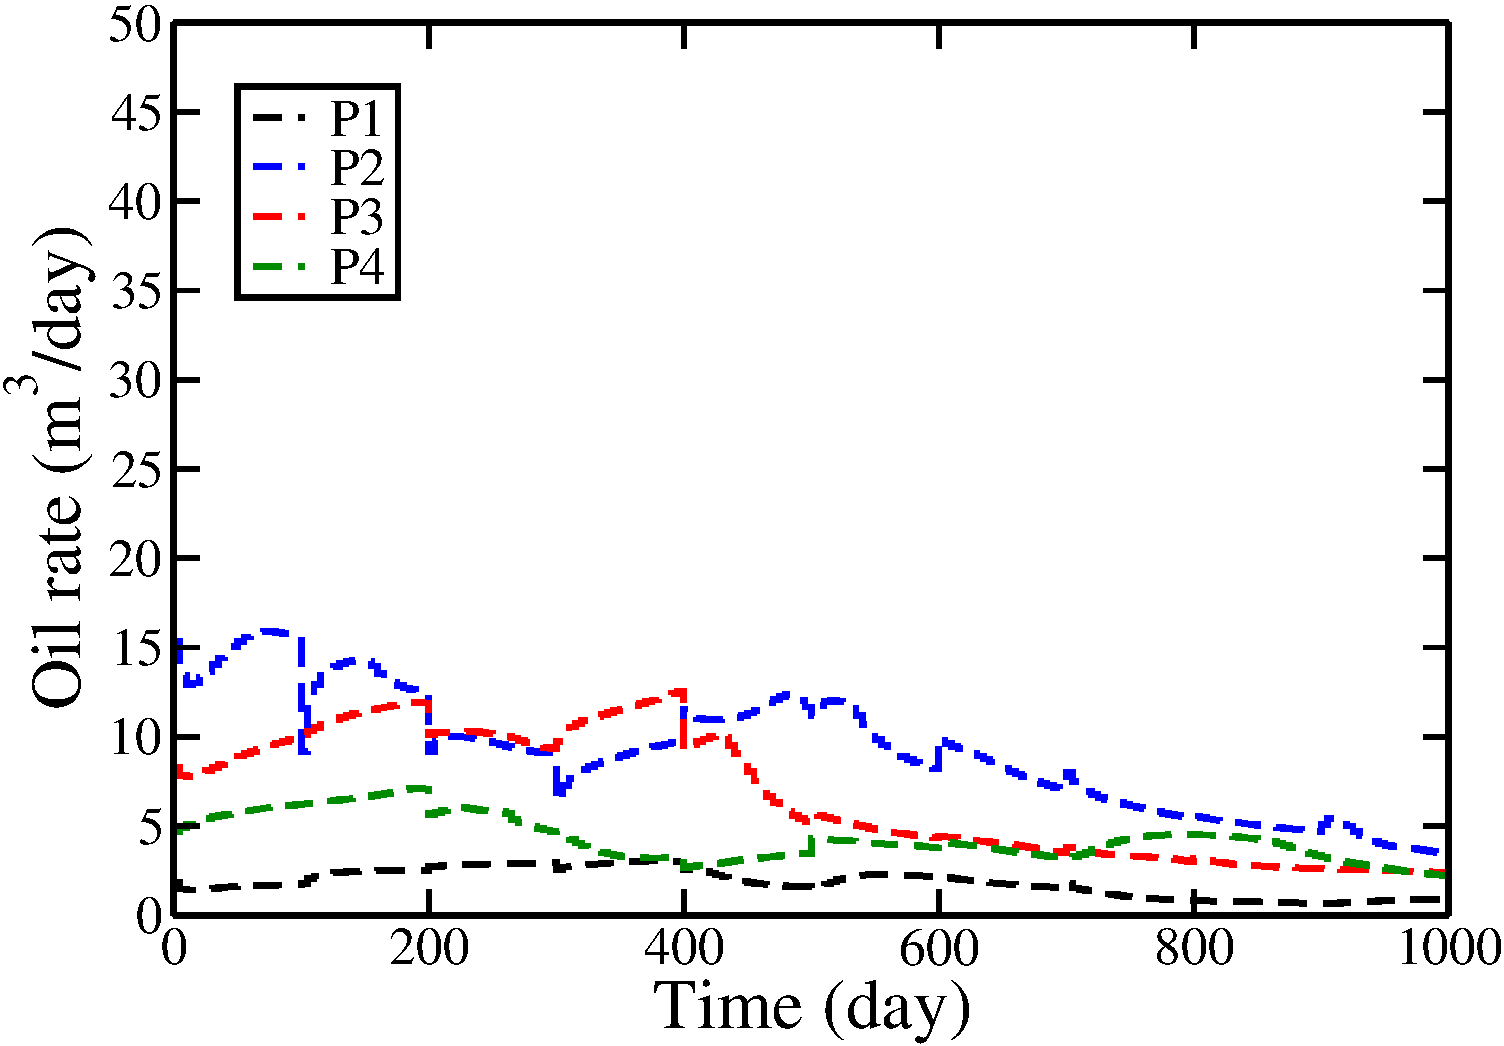
\includegraphics[totalheight=2.2in,angle=0]{figures/spe10topLayerOptimalChoppedIuPu_rate_oil.pdf}
\end{center}
\caption{BHPs (top), gas rates (middle) and oil rates
  (bottom) for the best heuristically constrained solution (Example 2, Run 9).}
\label{fig:SPE10TopLayerUnconstrainedOptimalChoppedRates}
\end{figure}
\begin{figure}
\begin{center}
\includegraphics[totalheight=2.2in,angle=0]{figures/spe10TopLayerConstrainedOptimalIuPa_BHP.pdf}
\includegraphics[totalheight=2.2in,angle=0]{figures/spe10TopLayerConstrainedOptimalIuPa_rate_gas.pdf}
\includegraphics[totalheight=2.2in,angle=0]{figures/spe10TopLayerConstrainedOptimalIuPa_rate_oil.pdf}
\end{center}
\caption{BHPs (top), gas rates (middle) and oil rates
  (bottom) for the best formally constrained solution (Example 2, Run 6).}
\label{fig:SPE10TopLayerConstrainedOptimalRates}
\end{figure}



\subsection{Example 3: Twelve-well channelized system}


Our third example uses the three-dimensional geological model introduced in
\cite{VanEssen}. We again consider CO$_2$ injection, though this model
contains a total of six components, defined in
Table~\ref{table:VanEssenModelFluid}. Further details are given in Table~\ref{table:VanEssenModelReservoir}.  A map of
the $x$-component of permeability (here $\tens{k}_x = \tens{k}_y = 10\tens{k}_z$), along with the
locations of the wells, is shown in Fig.~\ref{fig:VanEssenModelPermeabilityAndWells}.


\begin{figure}[ht]
     \begin{center}
      \begin{tabular}{cccccccc}
      53.90 & 108.0 & 216.5 & 433.9 & 569.6 & 1743 & 3493 & 7000 
      \end{tabular}
       \includegraphics[width=8cm,height=0.5cm]{figures/VanEssenModelPermeabilityMapColorBar.png}
                                                            
       \medskip
       
       \includegraphics[width=8cm]{figures/VanEssenModelPermeabilityMapConstant.png}%VanEssenModelPermeabilityMap.png}
%       \includegraphics[totalheight=10.5cm]{pdf/VanEssenModelPermeabilityXLogTransparent.pdf}
     \end{center}
     \caption{Reservoir model and wells for Example 3 (from \cite{VanEssen}). Background shows $\log \tens{k}_x$.}
  \label{fig:VanEssenModelPermeabilityAndWells}
\end{figure}



\begin{table}
\tabcolsep=0pt
\centering
\caption{Fluid description for example 2}
\begin{tabular*}{84mm}{@{\extracolsep\fill}lllllll}\toprule
Component            & CO$_2$ & C$_1$ & C$_2$ & C$_3$ & C$_4$  & C$_{10}$ \\[2pt]
\midrule
Initial comp. (\%)   & 1    & 20  & 30  & 19  & 10   & 20     \\
Injection comp. (\%) & 95   &  1  &  1  &  1  &  1   &  1     \\
\bottomrule
\end{tabular*}
\label{table:VanEssenModelFluid}
\end{table}


\begin{table}
\tabcolsep=0pt
\centering
\caption{Model parameters for example 2.}
\label{table:VanEssenModelReservoir}
\begin{tabular*}{84mm}{@{\extracolsep\fill}lll}\toprule
Parameter                      & Value           & Units     \\
\midrule
Grid size                      & 60 $\times$ 60 $\times$ 7 &  ---      \\
$\Delta x$                     & 24           & m            \\
$\Delta y$                     & 24           & m            \\
$\Delta z$                     &  4           & m            \\
Depth                          & 2538       & m              \\
Initial pressure               & 100          & bar          \\
Temperature                    & $372$     & $^\circ$C       \\
Rock compressibility           & $10^{-5}$    & 1 / bar      \\
Simulation time                & 300          & d            \\
Pressure upper bound           & 120          & bar          \\
Pressure lower bound           &  90          & bar          \\
Residual gas saturation  & 0 & ---                           \\
Residual oil saturation  & 0 & ---                           \\
End point rel perm gas   & 1 & ---                           \\
End point rel perm oil   & 1 & ---                           \\
Corey exponent gas       & 2 & ---                           \\
Corey exponent oil       & 2 & ---                           \\[2pt]
\bottomrule
Well locations [grid block no.] & $i$ & $j$                  \\
\midrule
Injector 1               &  5 &  57                          \\
Injector 2               &  30&  53                          \\
Injector 3               &   2&  35                          \\
Injector 4               &  27&  29                          \\
Injector 5               &  50&  35                          \\
Injector 6               &   8&   9                          \\
Injector 7               &  32&   2                          \\
Injector 8               &  57&   6                          \\
Producer 1               &  16&  43                          \\
Producer 2               &  35&  40                          \\
Producer 3               &  23&  16                          \\
Producer 4               &  43&  18                          \\[2pt]
\bottomrule
\end{tabular*}
\end{table}





The control parameters of our optimization problem are again the well BHPs.  The
wells are constrained to operate between an upper bound of 120~bar and a lower
bound of 90~bar. We also specify nonlinear constraints on both injection and
production in the form of maximum gas flow
rates of 200,000~m$^3/$d for the producers and 40,000~m$^3/$d for the injectors
(both at reservoir conditions). This model is run for a total of 100 days, and
we control the BHPs at initial time and then every ten days (the simulation time
frame is short in this case because the problem specification is such that oil
is produced quickly). There are a total of 120 control parameters in this
problem, and our objective is again to maximize cumulative oil production.

We simulate this model using the same procedures as in the previous examples.
Results for the nine runs for each case are presented in
Table~\ref{table:vanessen}. The feasible reference case yields 5.030$\times 10^6$~m$^3$ of
oil, while the best heuristically constrained case (Run~2) provides 5.457$\times 10^6$~m$^3$
of oil, an improvement of 8.5\%. The best formally constrained case (Run~3)
achieves an optimum of 5.306$\times 10^6$~m$^3$ of oil, which exceeds the reference case by
5.5\% but is less than the best heuristic case. The oil production profiles
for the best runs, along with the feasible reference case, are shown in
Fig.~\ref{fig:VanEssenRevenue}. We again see that the early time production in
the reference case exceeds that of the optimized cases, though the cumulative
oil produced in the optimized cases is of course higher. 

In this example, convergence of the optimizations using the formal constraint handling approach 
typically required about 48 forward simulations, while the heuristic treatment required only about 26. Our findings for this example clearly illustrate the potential advantages of the heuristic treatment for complex optimization problems involving multiple wells operating under nonlinear constraints.



\begin{table}
\centering
\caption{Oil production in $10^6$~m$^3$ (Example 3) for the optimized objective function
         without satisfying the nonlinear constraints (`Unconstr.'), satisfying the nonlinear constraints
         using the heuristic treatment (`Heuristic'), and satisfying the nonlinear constraints
         using the formal approach (`Formal'). Best feasible results shown in bold.}
\begin{tabular}{|c|c|c|c|}
\hline
 Run              & Unconstr. & Heuristic & Formal     \\
\hline
Reference         & 5.030 &  5.030    &          \\
1 & 5.450 &  5.449   &  5.284   \\
2 & 5.467 &\bf{5.457} &  5.294   \\
3 & 5.171 &  5.171   &\bf{5.306}\\
4 & 5.288 &  5.287   &  5.132   \\
5 & 5.424 &  5.423   &  5.224   \\
6 & 5.344 &  5.348   &  5.260   \\
7 & 5.321 &  5.230   &  4.994   \\
8 & 5.207 &  5.205   &  5.196   \\
9 & 5.353 &  5.349   &  4.986   \\
\hline
\end{tabular}
  \label{table:vanessen}
\end{table}


%1 & O30G23 5.450    &  5.2976    &  O41G30 5.284         \\
%2 & O47G27 5.467    &\bf{5.46} &  O46G30 5.294         \\
%3 & O22G12 5.171    &  5.02    &  O44G30 \bf{5.306}    \\
%4 & O25G18 5.288    &  5.02    &  O28G13 5.132         \\
%5 & O43G27 5.424    &  5.29    &  O35G30 5.224         \\
%6 & O43G19 5.344    &  5.35    &  O48G38 5.260         \\
%7 & O31G18 5.321    &  5.20    &  O43G29 4.994         \\
%8 & O19G10 5.207    &  5.21    &  O37G25 5.196         \\
%9 & O13G10 5.353    &  5.19    &  O91G26 4.986         \\


\begin{figure} [ht]
\begin{center}
\includegraphics[totalheight=2.2in,angle=0]{figures/vanEssenRevenue.pdf}
\end{center}
\caption{Oil production versus time for Example 3. Results are for
  feasible reference case (black curve), best heuristically constrained solution (Run 2, red curve)
  and best formally constrained solution (Run 3, blue curve).}
\label{fig:VanEssenRevenue}
\end{figure}



\section{Concluding remarks}  \label{sec:conclusions}
In this work we formulated and tested an adjoint-based optimization procedure
for compositional reservoir simulation. The method we employed was implemented into
Stanford's Automatic Differentiation-based General Purpose Research Simulator
(AD-GPRS). The use of automatic differentiation simplifies the adjoint
implementation and subsequent code enhancements. Two different treatments for
handling nonlinear constraints were presented. In the formal constraint handling
procedure, lumped constraints and their gradients are provided to the optimizer,
and feasibility is enforced by the optimization algorithm. In the second
(heuristic) procedure, an optimization satisfying only the bound and linear
constraints is performed first. Then, the forward model is run using the
controls from the first stage, but the simulator is allowed to switch from BHP
to rate control (for a problem in which BHPs are the control variables) as
required to satisfy the nonlinear rate constraints.


Numerical results were presented for four example cases of increasing
complexity. Nine runs, starting from different initial conditions, were
performed in all cases, for both the heuristic and the formal nonlinear
constraint treatments. In our examples, the control variables were the time-varying well BHPs, and maximum injection or production rate specifications entered as nonlinear
constraints. The total number of control variables ranged from 40 to 320. Improvement in cumulative oil produced (which was the objective function in all cases) using our optimization procedures ranged from 4.2\% to 11.6\% relative to the reference solutions. 

In the simplest case (Example~1), the formal constraint handling approach was shown to outperform the heuristic procedure when we increased the number of control variables from 40 to 320. In the next (somewhat more complicated) case, Example~2, the formal constraint treatment continued to outperform the heuristic procedure, though its advantage was very slight. In the other two cases, which were more challenging in terms of model size and number of wells (and they involved three-dimensional models, while the first two examples were two-dimensional), the heuristic treatment provided better objective function values than the formal approach. 

These observations suggest that, although the formal constraint handling approach is theoretically superior, complications related to constraint lumping and the existence of poor local optima (and the additional complexity inherent in problems with large numbers of optimization variables and nonlinear constraints) may render the formal procedure less effective than the heuristic approach in challenging cases. Thus, though we expect (and observe) the formal procedure to be the method of choice in relatively simple cases, the heuristic approach should be considered for use in more complex problems. It may even be beneficial to apply some type of hybrid technique, where the result from the heuristic method is used as the initial guess for the formal procedure. The use of a sequence of optimizations, with increasing numbers of control periods, should also be considered. Finally, it is important to note that the heuristic constraint treatment was found to be significantly more efficient than the formal approach. 


In addition to the discrete adjoint procedure, which was used for all of the
examples presented in this paper, we also derived and implemented a continuous
adjoint formulation. We showed that the two formulations use different
final time conditions and as a result the gradients do not
agree in general. However, the two boundary conditions become almost identical as the
size of the last time step approaches zero, in which case the gradients obtained by
both formulations are essentially the same.

There are a number of areas in which future research should be directed. Other
treatments for nonlinear constraints, both formal and heuristic, should be
considered, and the relative benefits of controlling rates instead of BHPs
should be assessed. It will be of interest to apply the general optimization
framework to larger and more realistic simulation models. Other types of wells
(horizontal, deviated, multilateral) should also be considered, along with the
optimization of downhole inflow control devices. The overall approach can be 
extended to perform robust control (to account for geological uncertainty) and hierarchical
(multi-objective) control to balance long-term and short-term objectives. Finally, our procedures could be applied for the optimization of CO$_2$ storage or for combined
EOR-CO$_2$ storage operations.



\section*{Acknowledgements}
We thank Denis Voskov and Oleg Volkov for useful discussions and assistance with AD-GPRS, and
Michael Saunders for his support 
on SNOPT. We are grateful
to the industrial affiliates of the Stanford University Smart Fields Consortium for partial
funding of this work.



